

%Exclusion limits on the generated SUSY \chono signal samples are derived at 95\% confidence level (CL) through the profile log-likelihood ratio test using the \(\mathrm{CL_S}\) prescription and performed with HistFitter.

The data are compared with the post-fit background expectations, derived from a background-only profile likelihood fit of all CRs and SRs simultaneously as described in Section~\ref{sec:stats}, and no significant excess is observed.
The VRs, shown in Figure~\ref{fig:dataMCagreement_CRVR}, demonstrate good modeling of the post-fit background expectation in regions kinematically similar to the SRs and for a variety of observables, validating the background-estimation technique.
The observed and expected numbers of events in \SRFR, \SRFour, and \SRThree are given in Table~\ref{tab:inclusive_SR_yields} 
inclusively and separated by the lepton flavor (electron or muon) of what would be the direct lepton from the \chone$\rightarrow$\Zboson$\ell$ decay.
The background expectation and uncertainty are further split into contributions from each category of SM processes.
Separate fits are performed for each flavor channel and for the inclusive channel, and therefore the predicted yields in the $e$ and $\mu$ channels may not necessarily add to the inclusive yield.
Note that for the \SRFR region, the electron and muon channels impose the same flavor requirement on both direct leptons in the event, and so the yield in the $\text{SRFR}_{e}$ and $\text{SRFR}_{\mu}$ regions do not add to the inclusive \SRFR region.

\begin{table}
\caption[The observed yields and post-fit background expectations in \SRTL, \SRFour, and \SRThree, shown inclusively and when the direct lepton from a \chono decay is required to be an electron or muon.]{
  The observed yields and post-fit background expectations in \SRTL, \SRFour, and \SRThree, shown inclusively and when the direct lepton from a \chono decay is required to be an electron or muon.
  \captionlegend
  Uncertainties in the background expectation include combined statistical and systematic uncertainties.
  The individual uncertainties may be correlated and do not necessarily combine in quadrature to give the total background uncertainty.
}
\label{tab:inclusive_SR_yields}
  \begin{center}
  \setlength{\tabcolsep}{0.0pc}
  {\small
  %%
\begin{tabular*}{\textwidth}{@{\extracolsep{\fill}}lcccccc}
\noalign{\smallskip}\hline\noalign{\smallskip}
{Region}                    & \SRTL                            & \SRTLE                           & \SRTLM                           & \SRFour                             & \SRFourE                            & \SRFourM   \\
\noalign{\smallskip}\hline\noalign{\smallskip}
 Observed yield             & $42$                                & $15$                                & $17$                                & $89$                                & $48$                                & $41$   \\
\noalign{\smallskip}\hline\noalign{\smallskip}
 Expected background yield  & $\phantom{}39 \pm 4\phantom{0}$ & $\phantom{}13.7 \pm 2.0\phantom{0}$ & $\phantom{}15.7 \pm 2.5\phantom{0}$ & $\phantom{.0}76 \pm 6\phantom{.00}$ & $\phantom{.0}35.8 \pm 3.5\phantom{.00}$ & $\phantom{}38.2 \pm 2.8\phantom{0}$ \\
\noalign{\smallskip}\hline\noalign{\smallskip}
 $WZ$ yield                 & $-$                                 & $-$                                 & $-$                                 & $-$                                 & $-$                                 & $-$         \\
 $ZZ$ yield                 & $\phantom{}19 \pm 4\phantom{0}$     & $7.1 \pm 1.7$                       & $\phantom{}10.4 \pm 2.4\phantom{0}$ & $\phantom{}20.9 \pm 1.1\phantom{0}$ & $9.5 \pm 0.6$                       & $\phantom{}11.2 \pm 0.7\phantom{0}$ \\
 $t\bar{t}Z$ yield          & $\phantom{}12.2 \pm 3.2\phantom{0}$ & $2.4 \pm 0.7$                       & $3.0 \pm 0.6$                       & $\phantom{.0}18 \pm 6\phantom{.00}$ & $9.1 \pm 3.2$                       & $8.5 \pm 1.6$         \\
 Triboson yield             & $1.3 \pm 0.4$                       & $0.25 \pm 0.09$                     & $0.33 \pm 0.12$                     & $\phantom{}12.2 \pm 2.8\phantom{0}$ & $5.8 \pm 1.4$                       & $6.0 \pm 1.5$  \\
 Higgs yield                & $2.6 \pm 0.5$                       & $0.72 \pm 0.17$                     & $1.17 \pm 0.25$                     & $\phantom{}11.2 \pm 2.0\phantom{0}$ & $5.3 \pm 1.0$                       & $5.5 \pm 1.1$ \\
 Other yield                & $2.1 \pm 0.5$                       & $0.25 \pm 0.17$                     & $0.39 \pm 0.16$                     & $7.9 \pm 1.5$                       & $4.0 \pm 0.8$                       & $3.5 \pm 0.8$          \\
 \emph{Fake} yield          & $1.3 \pm 0.8$                       & $3.0 \pm 1.5$                       & $0.5_{-0.5}^{+0.6}$~                 & $6.4 \pm 2.5$                       & $2.1 \pm 1.1$                       & $3.6 \pm 1.7$          \\
\noalign{\smallskip}\hline\noalign{\smallskip}
 {Region}                   & \SRThree                            & \SRThreeE                           & \SRThreeM                              & & & \\[-0.05cm]
\noalign{\smallskip}\hline\noalign{\smallskip}
 Observed yield             & $61$                                & $28$                                & $33$                                & & & \\
\noalign{\smallskip}\hline\noalign{\smallskip}
 Expected background yield  & $\phantom{}54.9 \pm 3.3\phantom{0}$ & $\phantom{}27.5 \pm 2.2\phantom{0}$ & $\phantom{}27.4 \pm 2.0\phantom{0}$ & & & \\
\noalign{\smallskip}\hline\noalign{\smallskip}
 $WZ$ yield                 & $\phantom{}33.6 \pm 2.4\phantom{0}$ & $\phantom{}16.5 \pm 1.7\phantom{0}$ & $\phantom{}17.3 \pm 1.8\phantom{0}$ & & & \\
 $ZZ$ yield                 & $0.92 \pm 0.27$                     & $0.11 \pm 0.04$                     & $0.77 \pm 0.24$                     & & & \\
 $t\bar{t}Z$ yield          & $7.5 \pm 2.3$                       & $4.1 \pm 1.3$                       & $3.4 \pm 0.7$                       & & & \\
 Triboson yield             & $5.6 \pm 1.5$                       & $2.7 \pm 0.8$                       & $2.6 \pm 0.7$                       & & & \\
 Higgs yield                & $0.51 \pm 0.10$                     & $0.25 \pm 0.06$                     & $0.23 \pm 0.05$                     & & & \\
 Other yield                & $4.2 \pm 0.8$                       & $2.0 \pm 0.4$                       & $2.0 \pm 0.4$                       & & & \\
 \emph{Fake} yield          & $2.5 \pm 1.2$                       & $1.8 \pm 1.1$                       & $1.0 \pm 0.8$                       & & & \\
\noalign{\smallskip}\hline\noalign{\smallskip}
\end{tabular*}
%%%
}
\end{center}
 

\end{table}

The \mZl distributions in each SR, with binning corresponding to that used in the fit, are shown in Figure~\ref{fig:mZl}.
The SRs show good agreement in the shape of the \mZl distribution between data and the background prediction, with no significant localized excesses.
Three example signals of mass 200, 500, and 800~\GeV are included in these figures and peak strongly in their target \mZl bin for all three SRs, with the 800~\GeV signal only visible in the last \mZl bin.
%Other observables in the SRs relevant for the extrapolation of the yield normalization are shown in Figure~\ref{fig:SR_dist} and also demonstrate good agreement.

\subsection{Model-Independent Limits on New Physics in Inclusive Regions}
%Each bin of the \mZl distribution in each SR is fit independently resulting in 48 SRs being fit simultaneously.
%The modified frequentist \(\mathrm{CL_S}\) technique described in Section %\ref{sec:stats:CLs} is then used to determine the expected mass limit. 
%The wino mass limit for the branching ratio being tested is selected as the point where \(\mathrm{CL_S}\) = 0.05.

Via the model-independent fit procedure detailed in Section \ref{sec:stats:modind} and the modified frequentist \(\mathrm{CL_S}\) technique described in Section \ref{sec:stats:CLs}, upper limits are set on the possible visible cross sections of generic beyond-the-SM (BSM) processes in each \mZl bin of each SR.
%The wino mass limit for the branching ratio being tested is selected as the point where \(\mathrm{CL_S}\) = 0.05.
%These model-independent limits are derived at 95\% confidence level (CL) using the \CLs prescription~\cite{Read:2002hq},
%and results are evaluated using pseudo-experiments.
%A profile likelihood fit is performed on the numbers of observed and expected events in the target \mZl bin of one SR and the three CRs,
A generic BSM process is assumed to contribute only to the target \mZl bin.
In this way no assumption is made concerning the \chono branching fractions or \mZl shape of the BSM process.
No uncertainties in the yield of the BSM process are considered, except for the luminosity uncertainty.

This procedure is repeated for each of the 16 \mZl bins in each of the three SRs, with only one SR bin considered for each fit.
This differs from the nominal fit strategy which is performed using the three CRs and the 48 \mZl bins of the SRs simultaneously,
though only minor differences from the significances shown in the bottom panel of Figure~\ref{fig:mZl} are seen.
\begin{figure}[ht]
    \centering
    \begin{subfigure}[b]{0.49\textwidth}
      \centering
      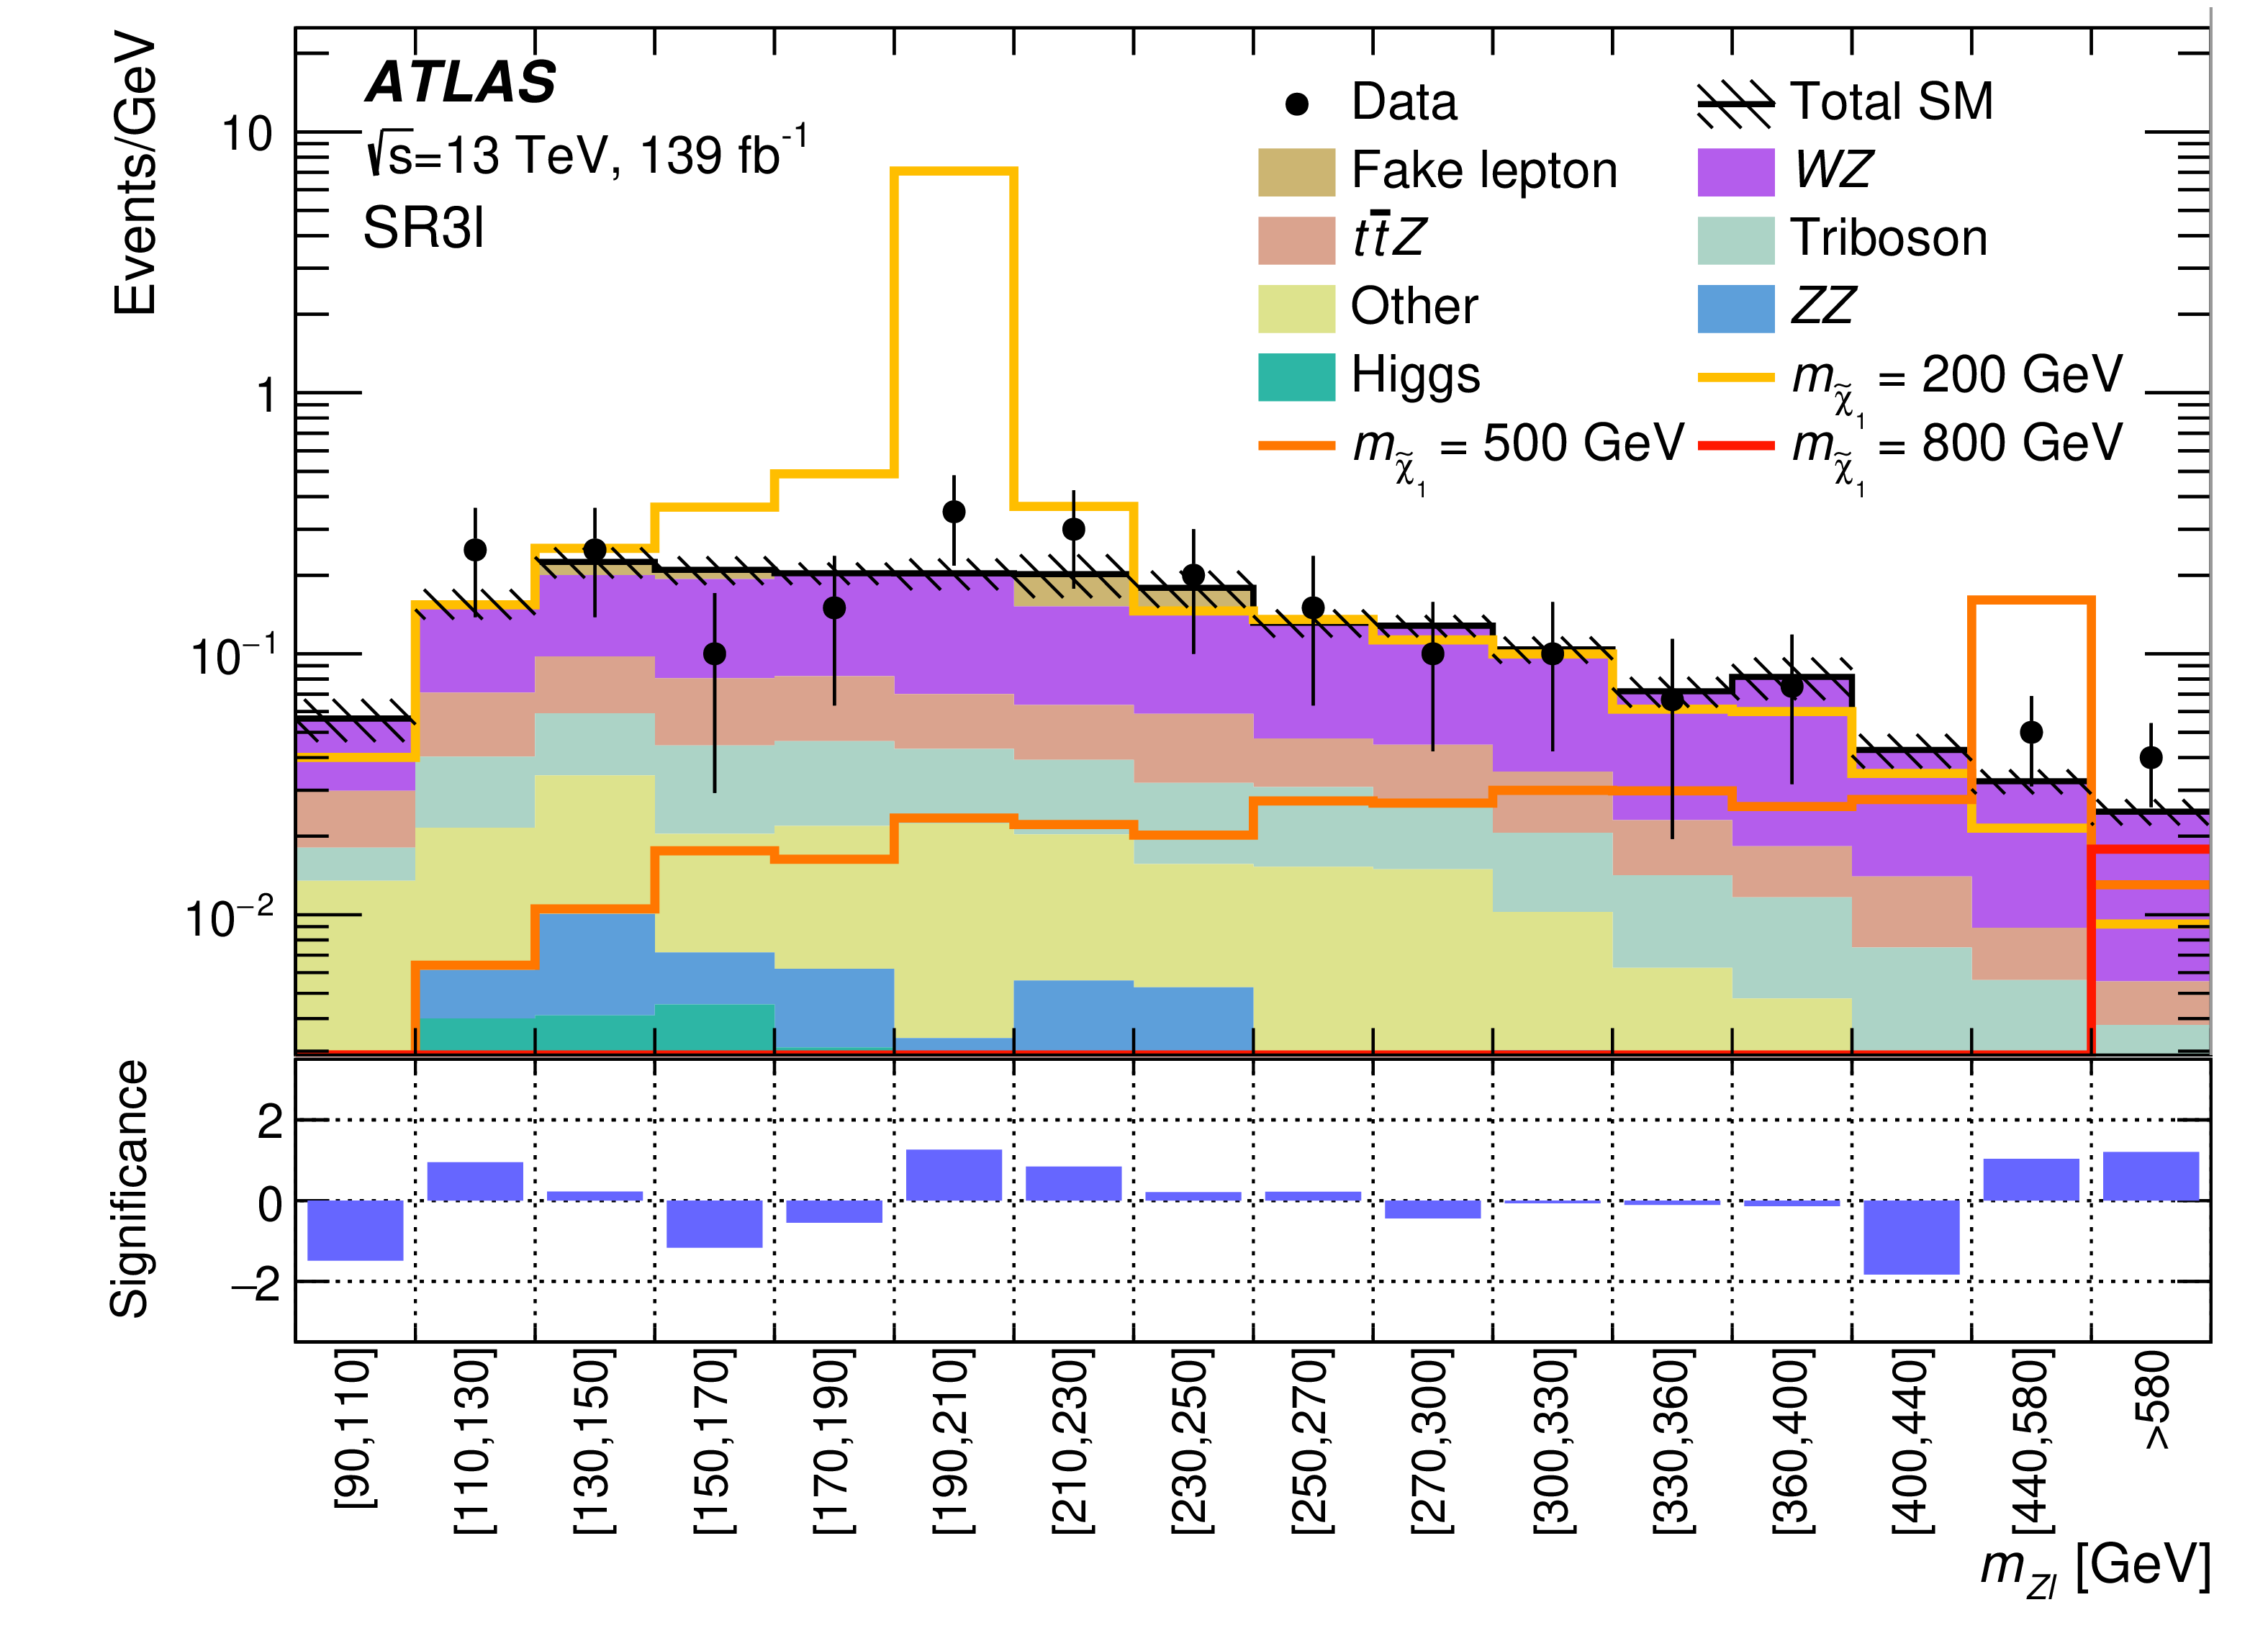
\includegraphics[width=0.98\textwidth]{figs/rpvthreel/histpull_all_doSRsInBkg_SROL3l.png}
      \caption{}
      \label{fig:mZl_SR3l}
    \end{subfigure}
    \hfill
    \begin{subfigure}[b]{0.49\textwidth}
      \centering
      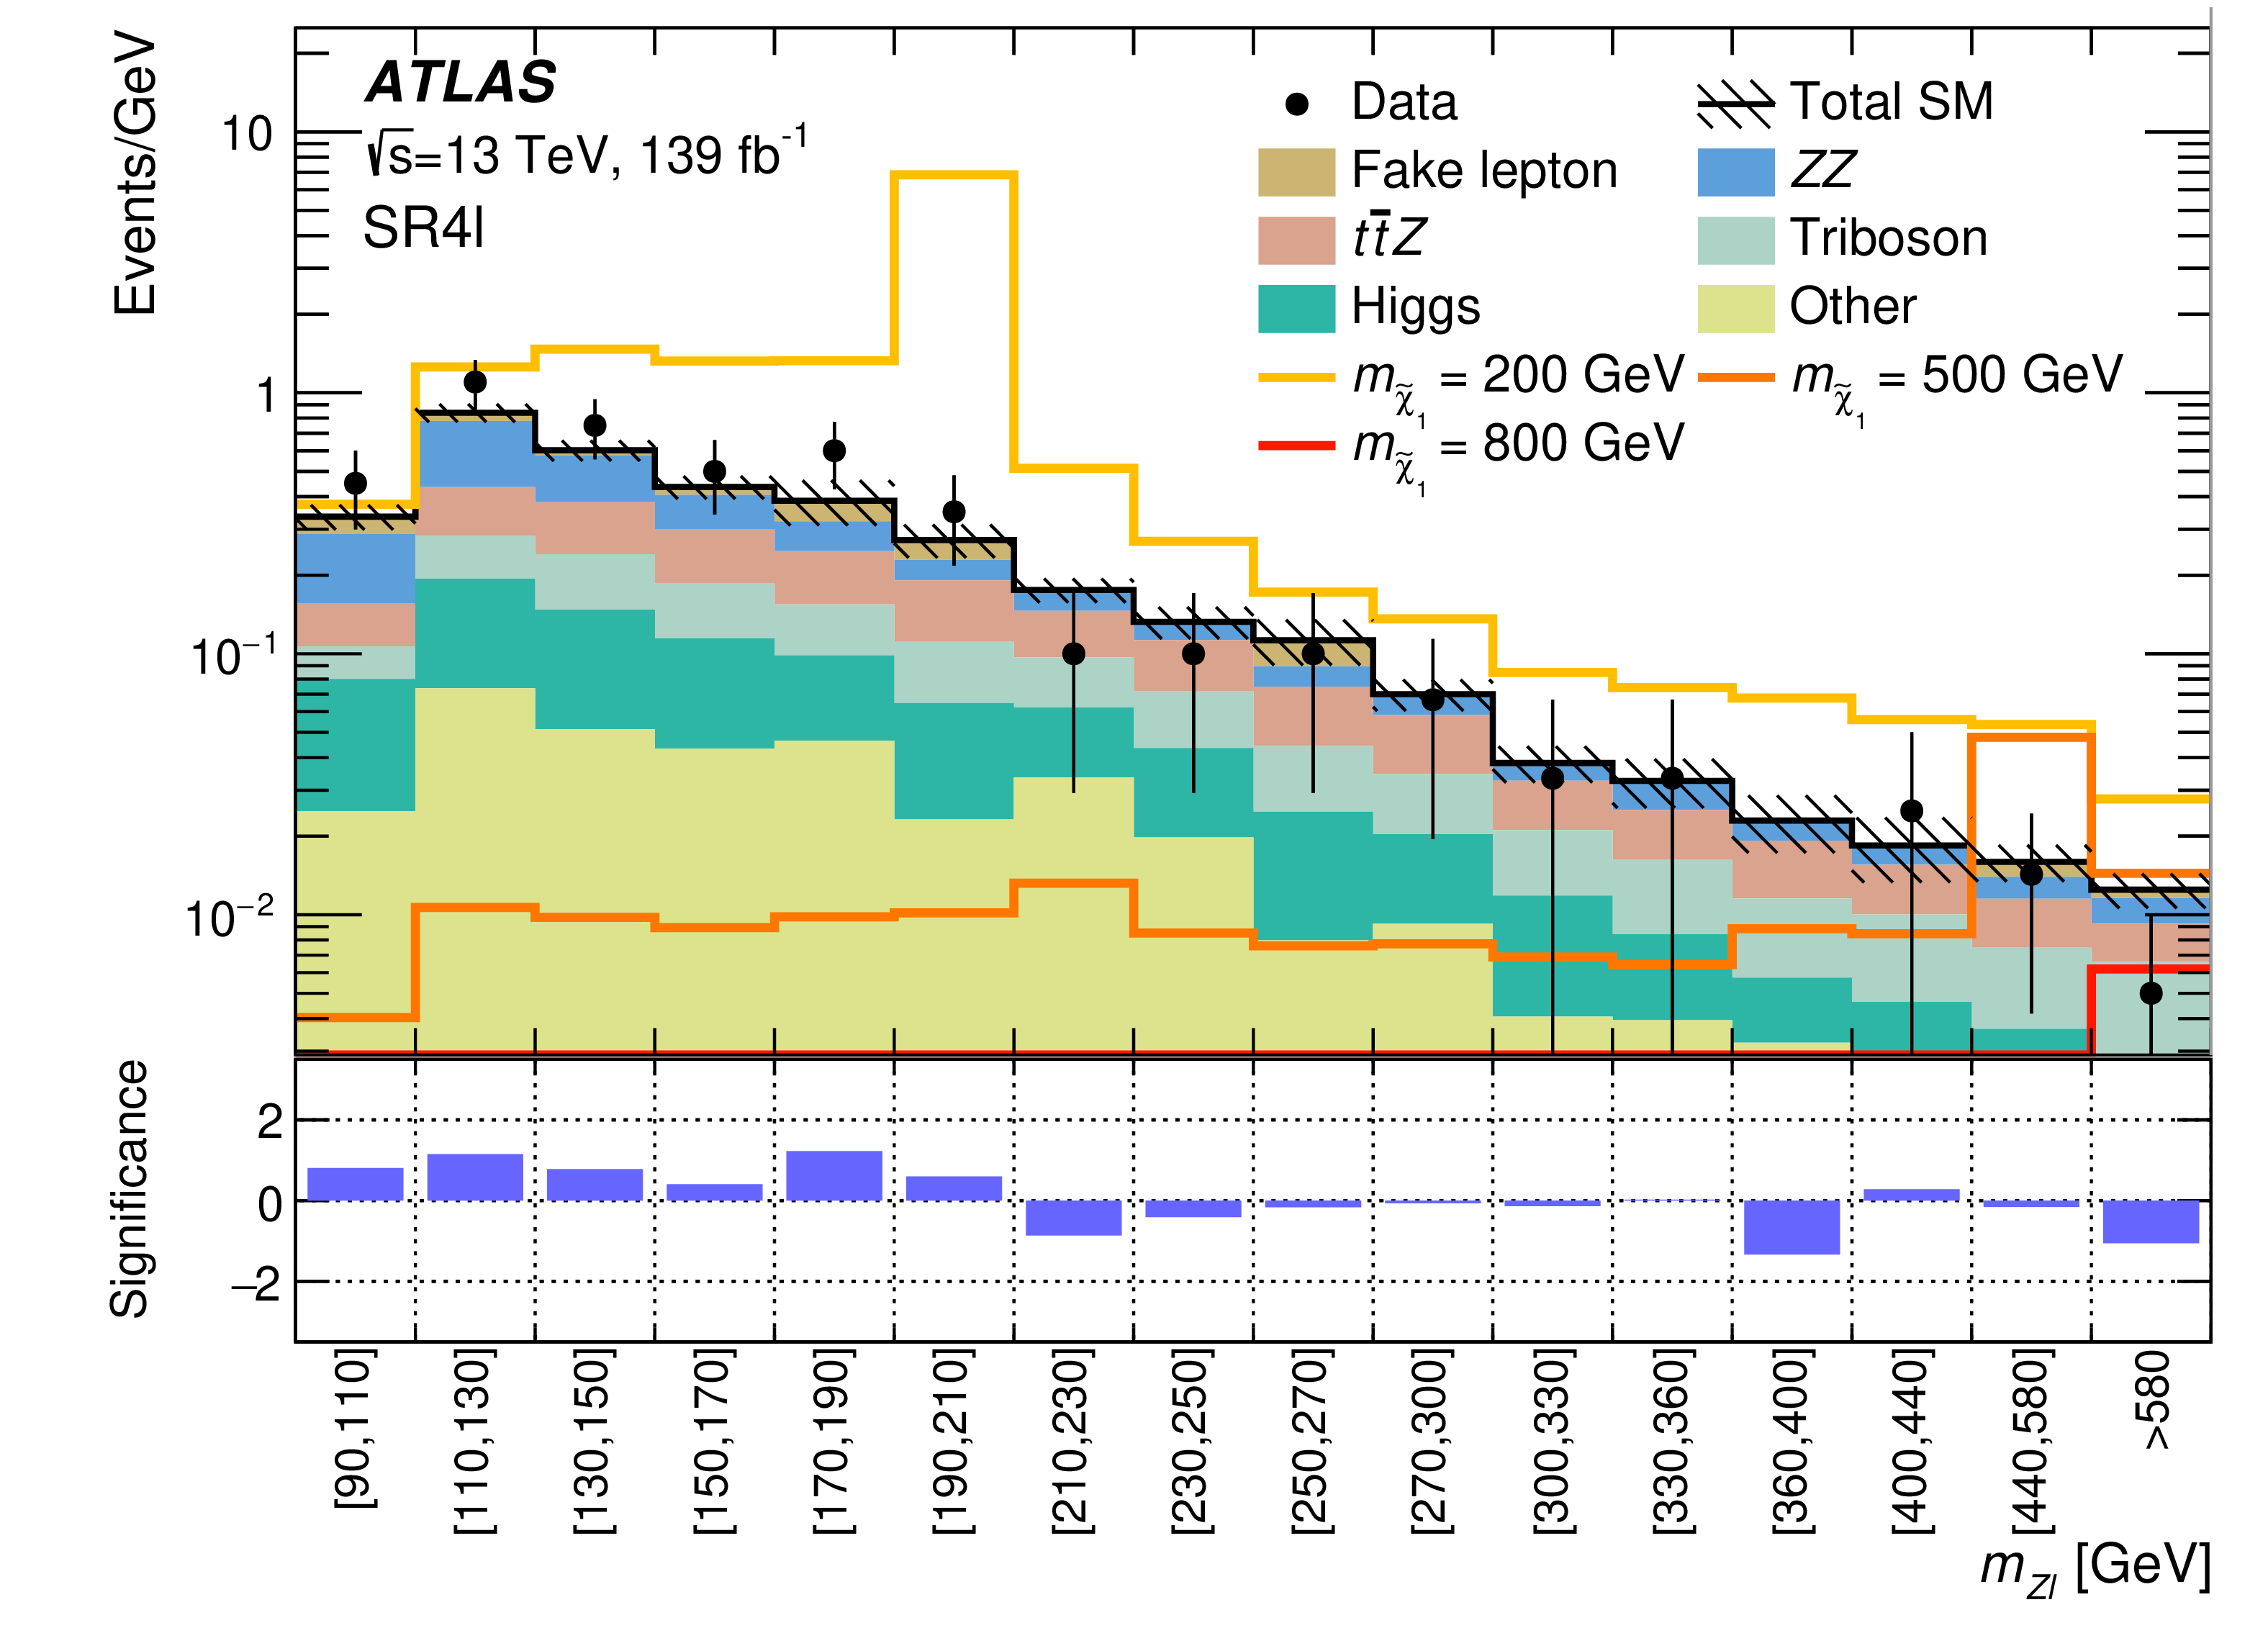
\includegraphics[width=0.98\textwidth]{figs/rpvthreel/histpull_all_doSRsInBkg_SROL4l.png}
      \caption{}
      \label{fig:mZl_SR4l}
    \end{subfigure}
    \hfill
    \begin{subfigure}[b]{0.49\textwidth}
      \centering
      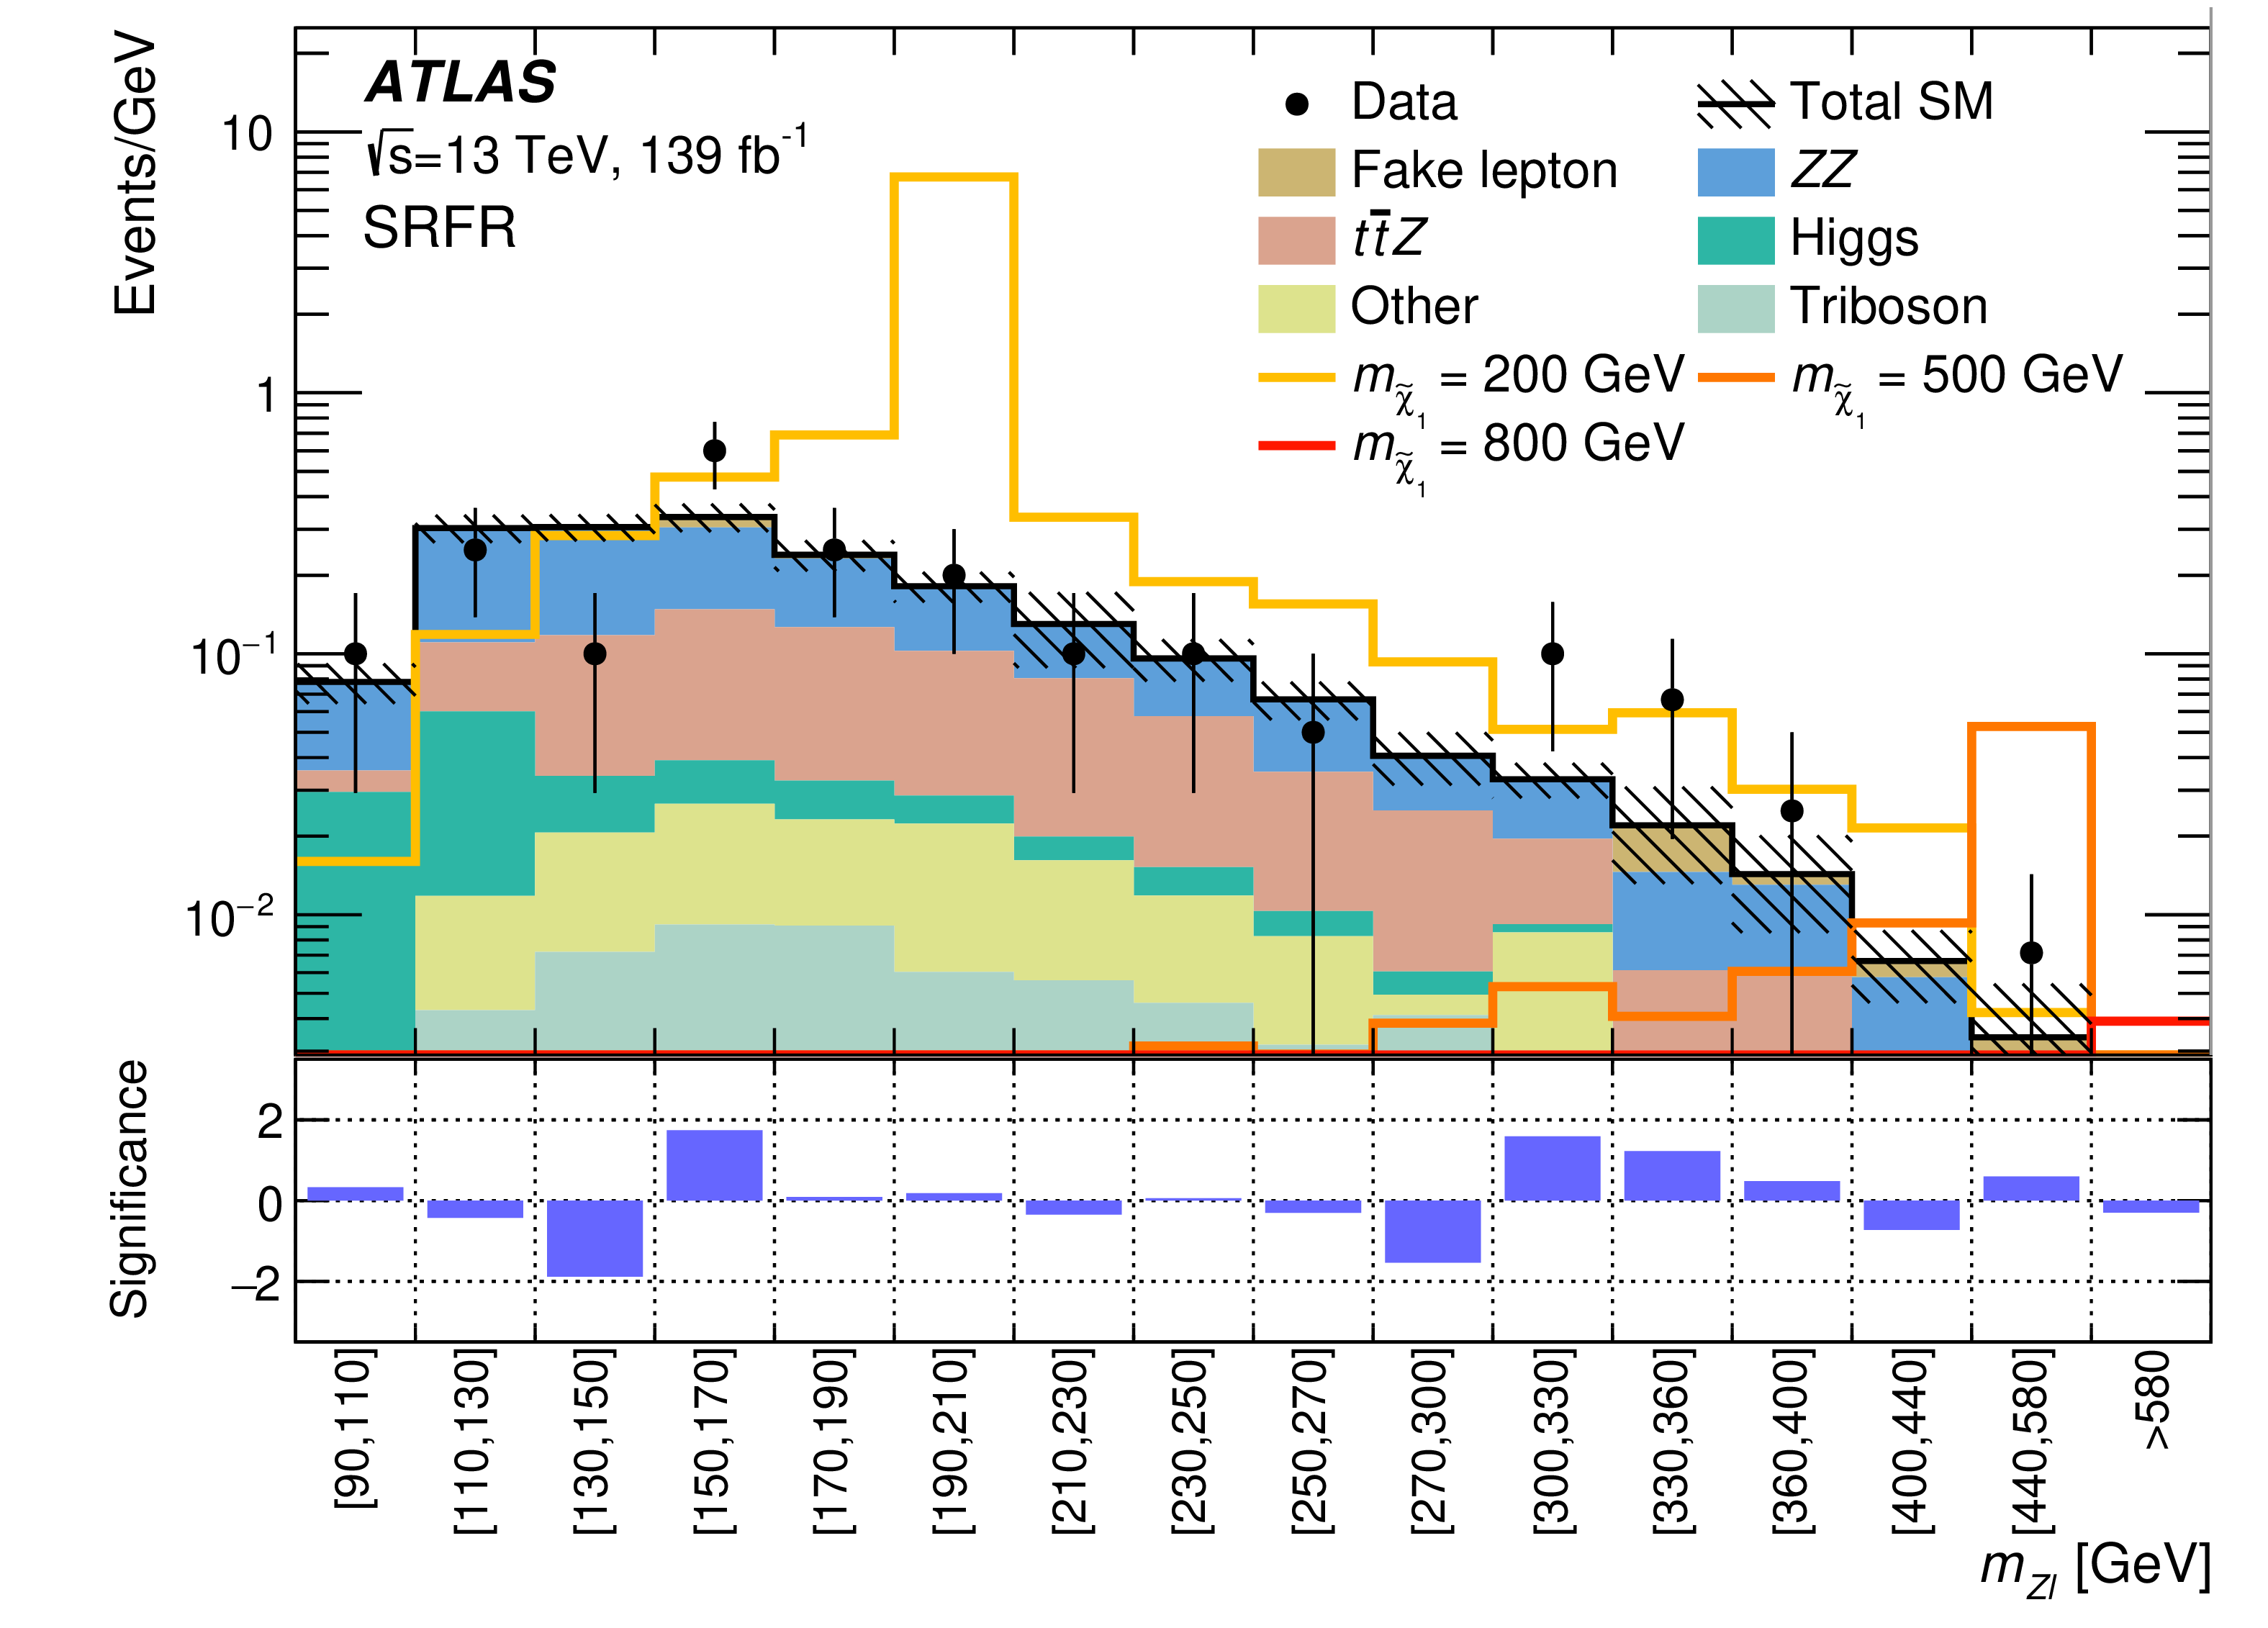
\includegraphics[width=0.98\textwidth]{figs/rpvthreel/histpull_all_doSRsInBkg_SRTL.png}
      \caption{}
      \label{fig:mZl_SRFR}
    \end{subfigure}
    \caption[The observed data and post-fit SM background expectation as a function of \mZl in \SRTL, \SRFour, and \SRThree]{The observed data and post-fit SM background expectation as a function of \mZl in (top left) \SRTL, (top right) \SRFour, and (bottom) \SRThree.
    The \mZl binning (Eq.~(\ref{eq:binning})) is the same as that used in the fit and the yield is normalized to the bin width, with the last bin normalized using a width of 200~\GeV. 
    \captionlegend
    \captionsysband
    The bottom panel shows the significance of the differences between the observed data and expected yields,
    computed following the profile likelihood method described in Ref.~\cite{Cousins:2007bmb}
    \cite{ATLAS:2020uer}.}
    \label{fig:mZl}
\end{figure}

\subsection{Mass limits on \BL RPV production}
%\textcolor{red}{\hrulefill \textsc{Unfinished Section}\hrulefill}  \\
Exclusion limits on the generated SUSY \chono signal samples are derived at 95\% confidence level (CL) through the profile log-likelihood ratio test using the \(\mathrm{CL_S}\) prescription and performed with \Histfitter.
For each signal model, a simultaneous fit is performed to the control regions and the signal regions, fitting to the number of events passing each selection criteria. 
Each bin of the \mZl distribution in each SR is fit independently, so there are effectively 48 SRs being fit simultaneously.
The modified frequentist \(\mathrm{CL_S}\) technique is then used to determine the expected mass limit. 
The wino mass limit for the branching ratio being tested is selected as the point where \(\mathrm{CL_S}\) = 0.05.
The mass points sampled are from 100~\GeV to 1500~\GeV in steps of 50~\GeV.

\begin{figure}
    \centering
    \begin{subfigure}[b]{0.49\textwidth}
      \centering
      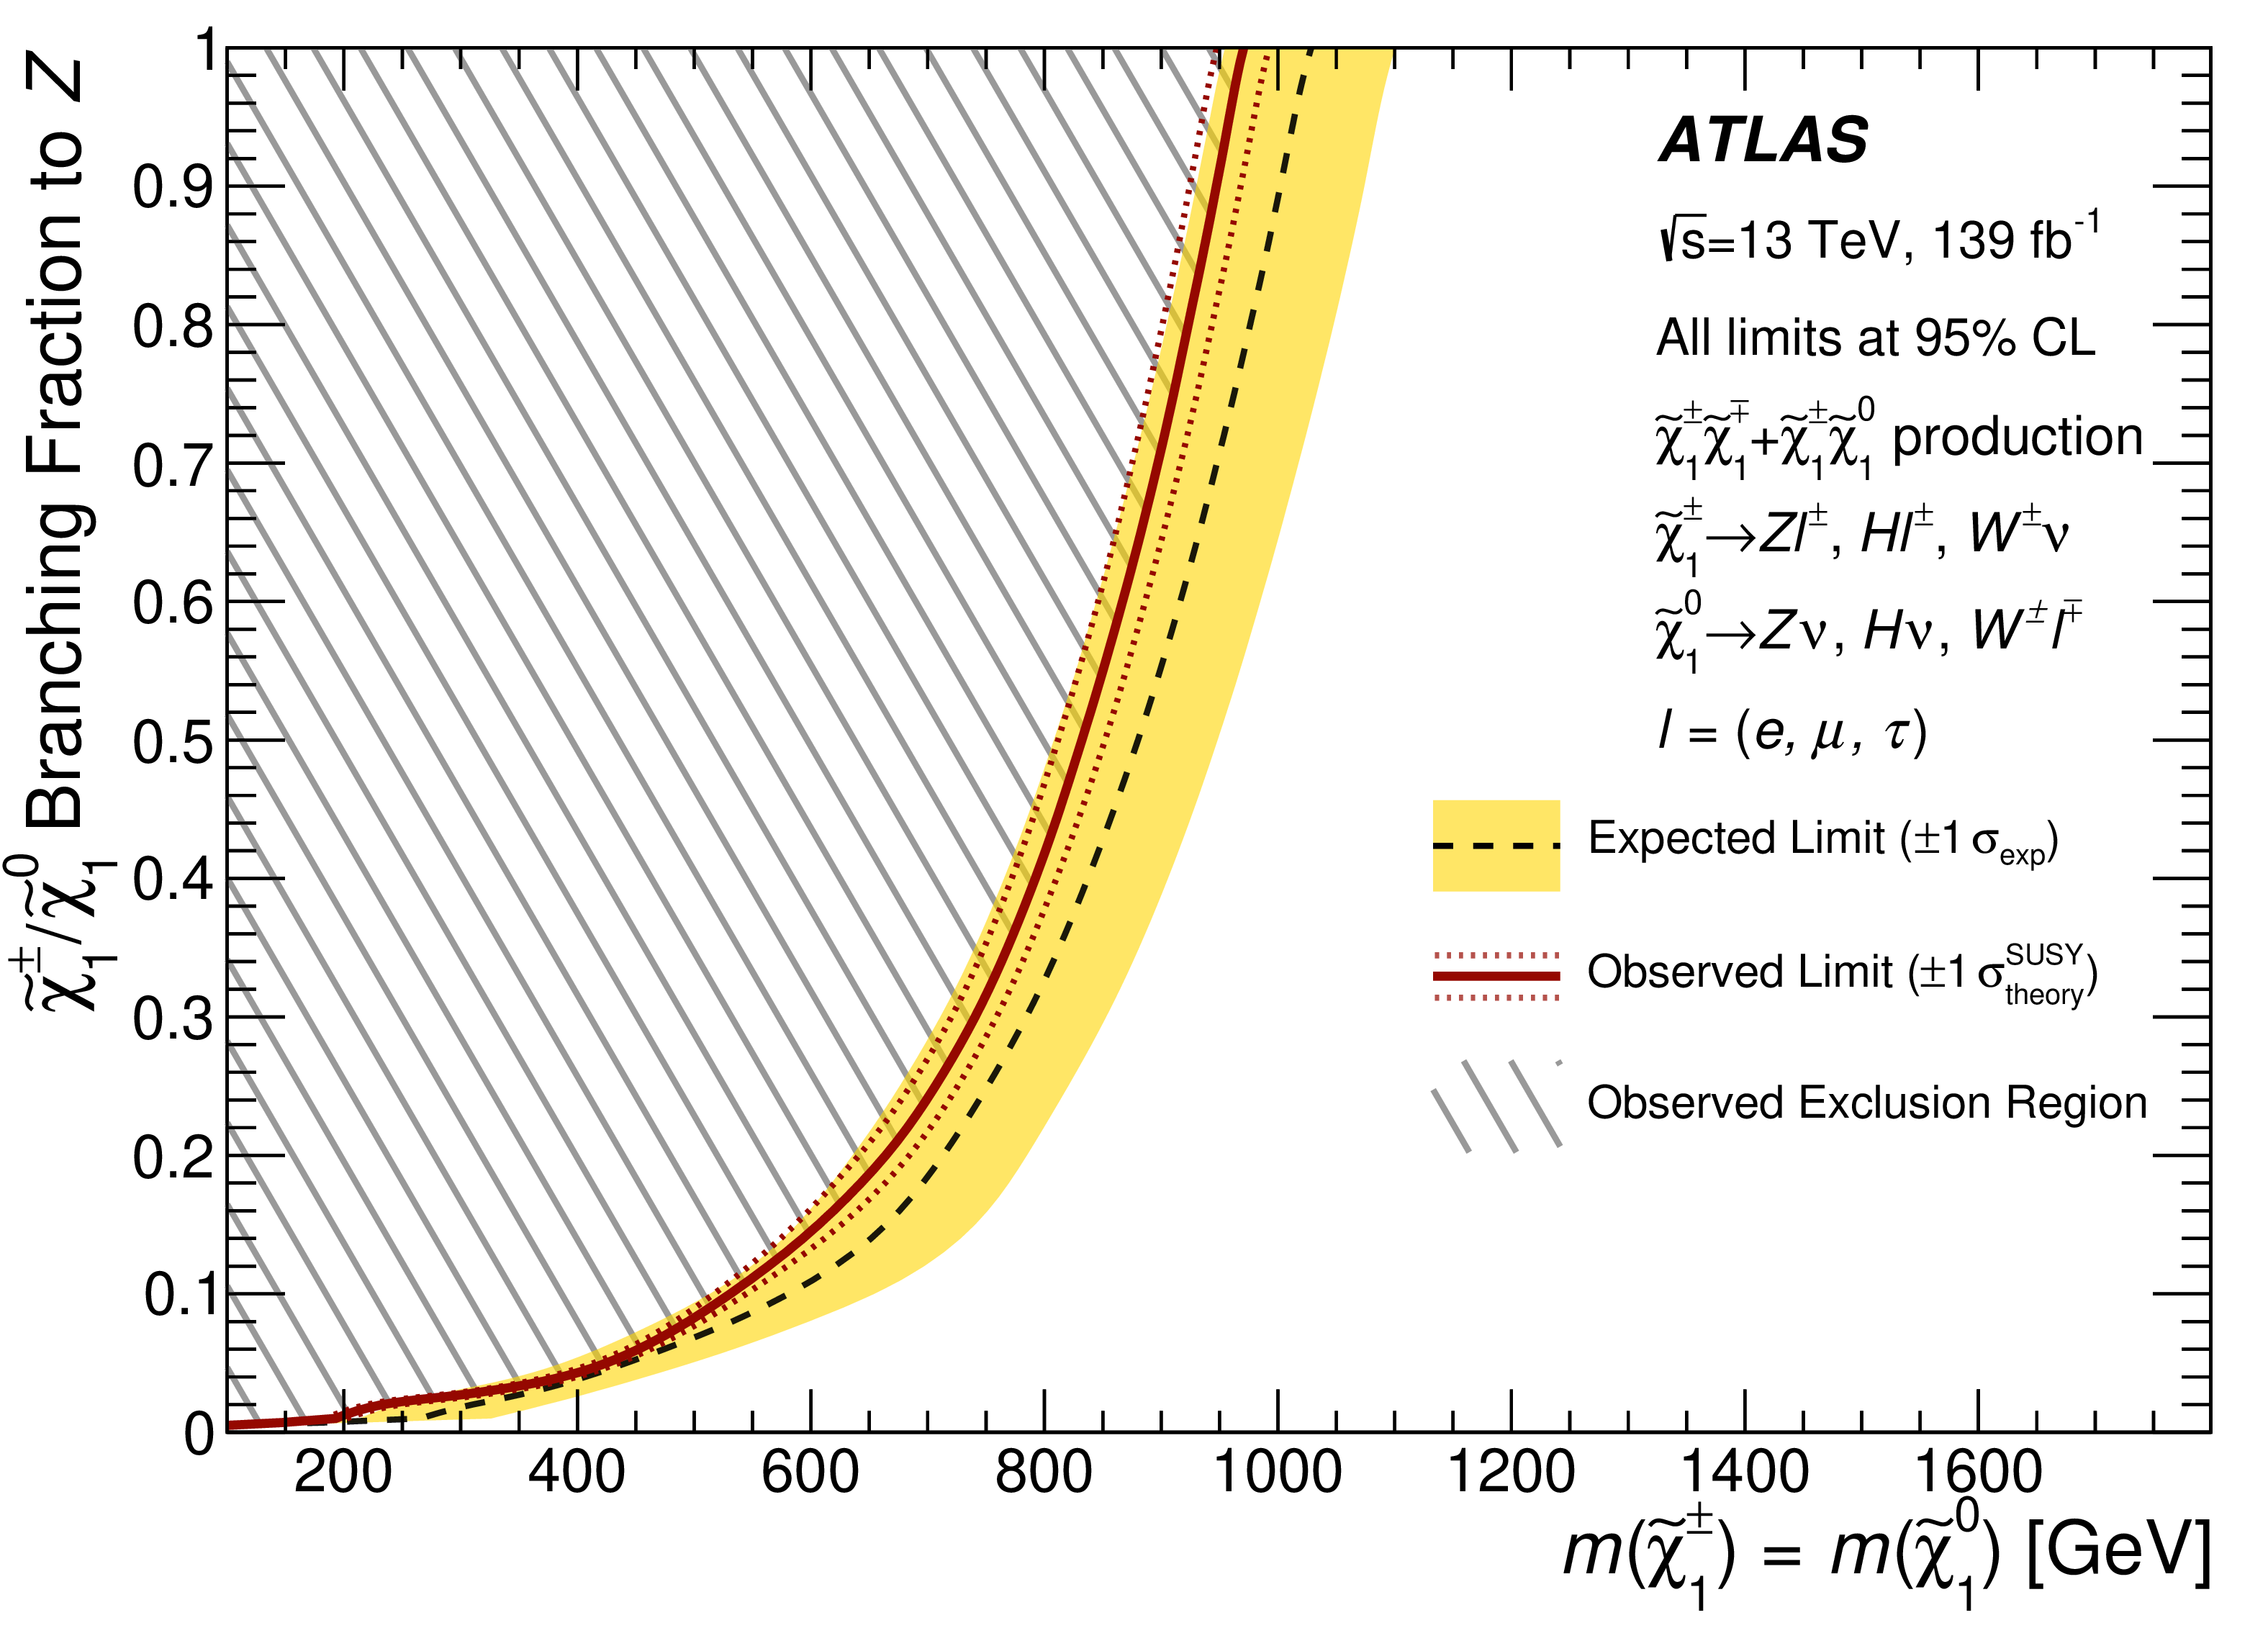
\includegraphics[width=0.98\textwidth]{figs/rpvthreel/contours_bre_33_brm_33_brt_33_Nominal.png}
      \caption{}
      \label{fig:contour_democratic}
    \end{subfigure}
    \hfill
    \begin{subfigure}[b]{0.49\textwidth}
      \centering
      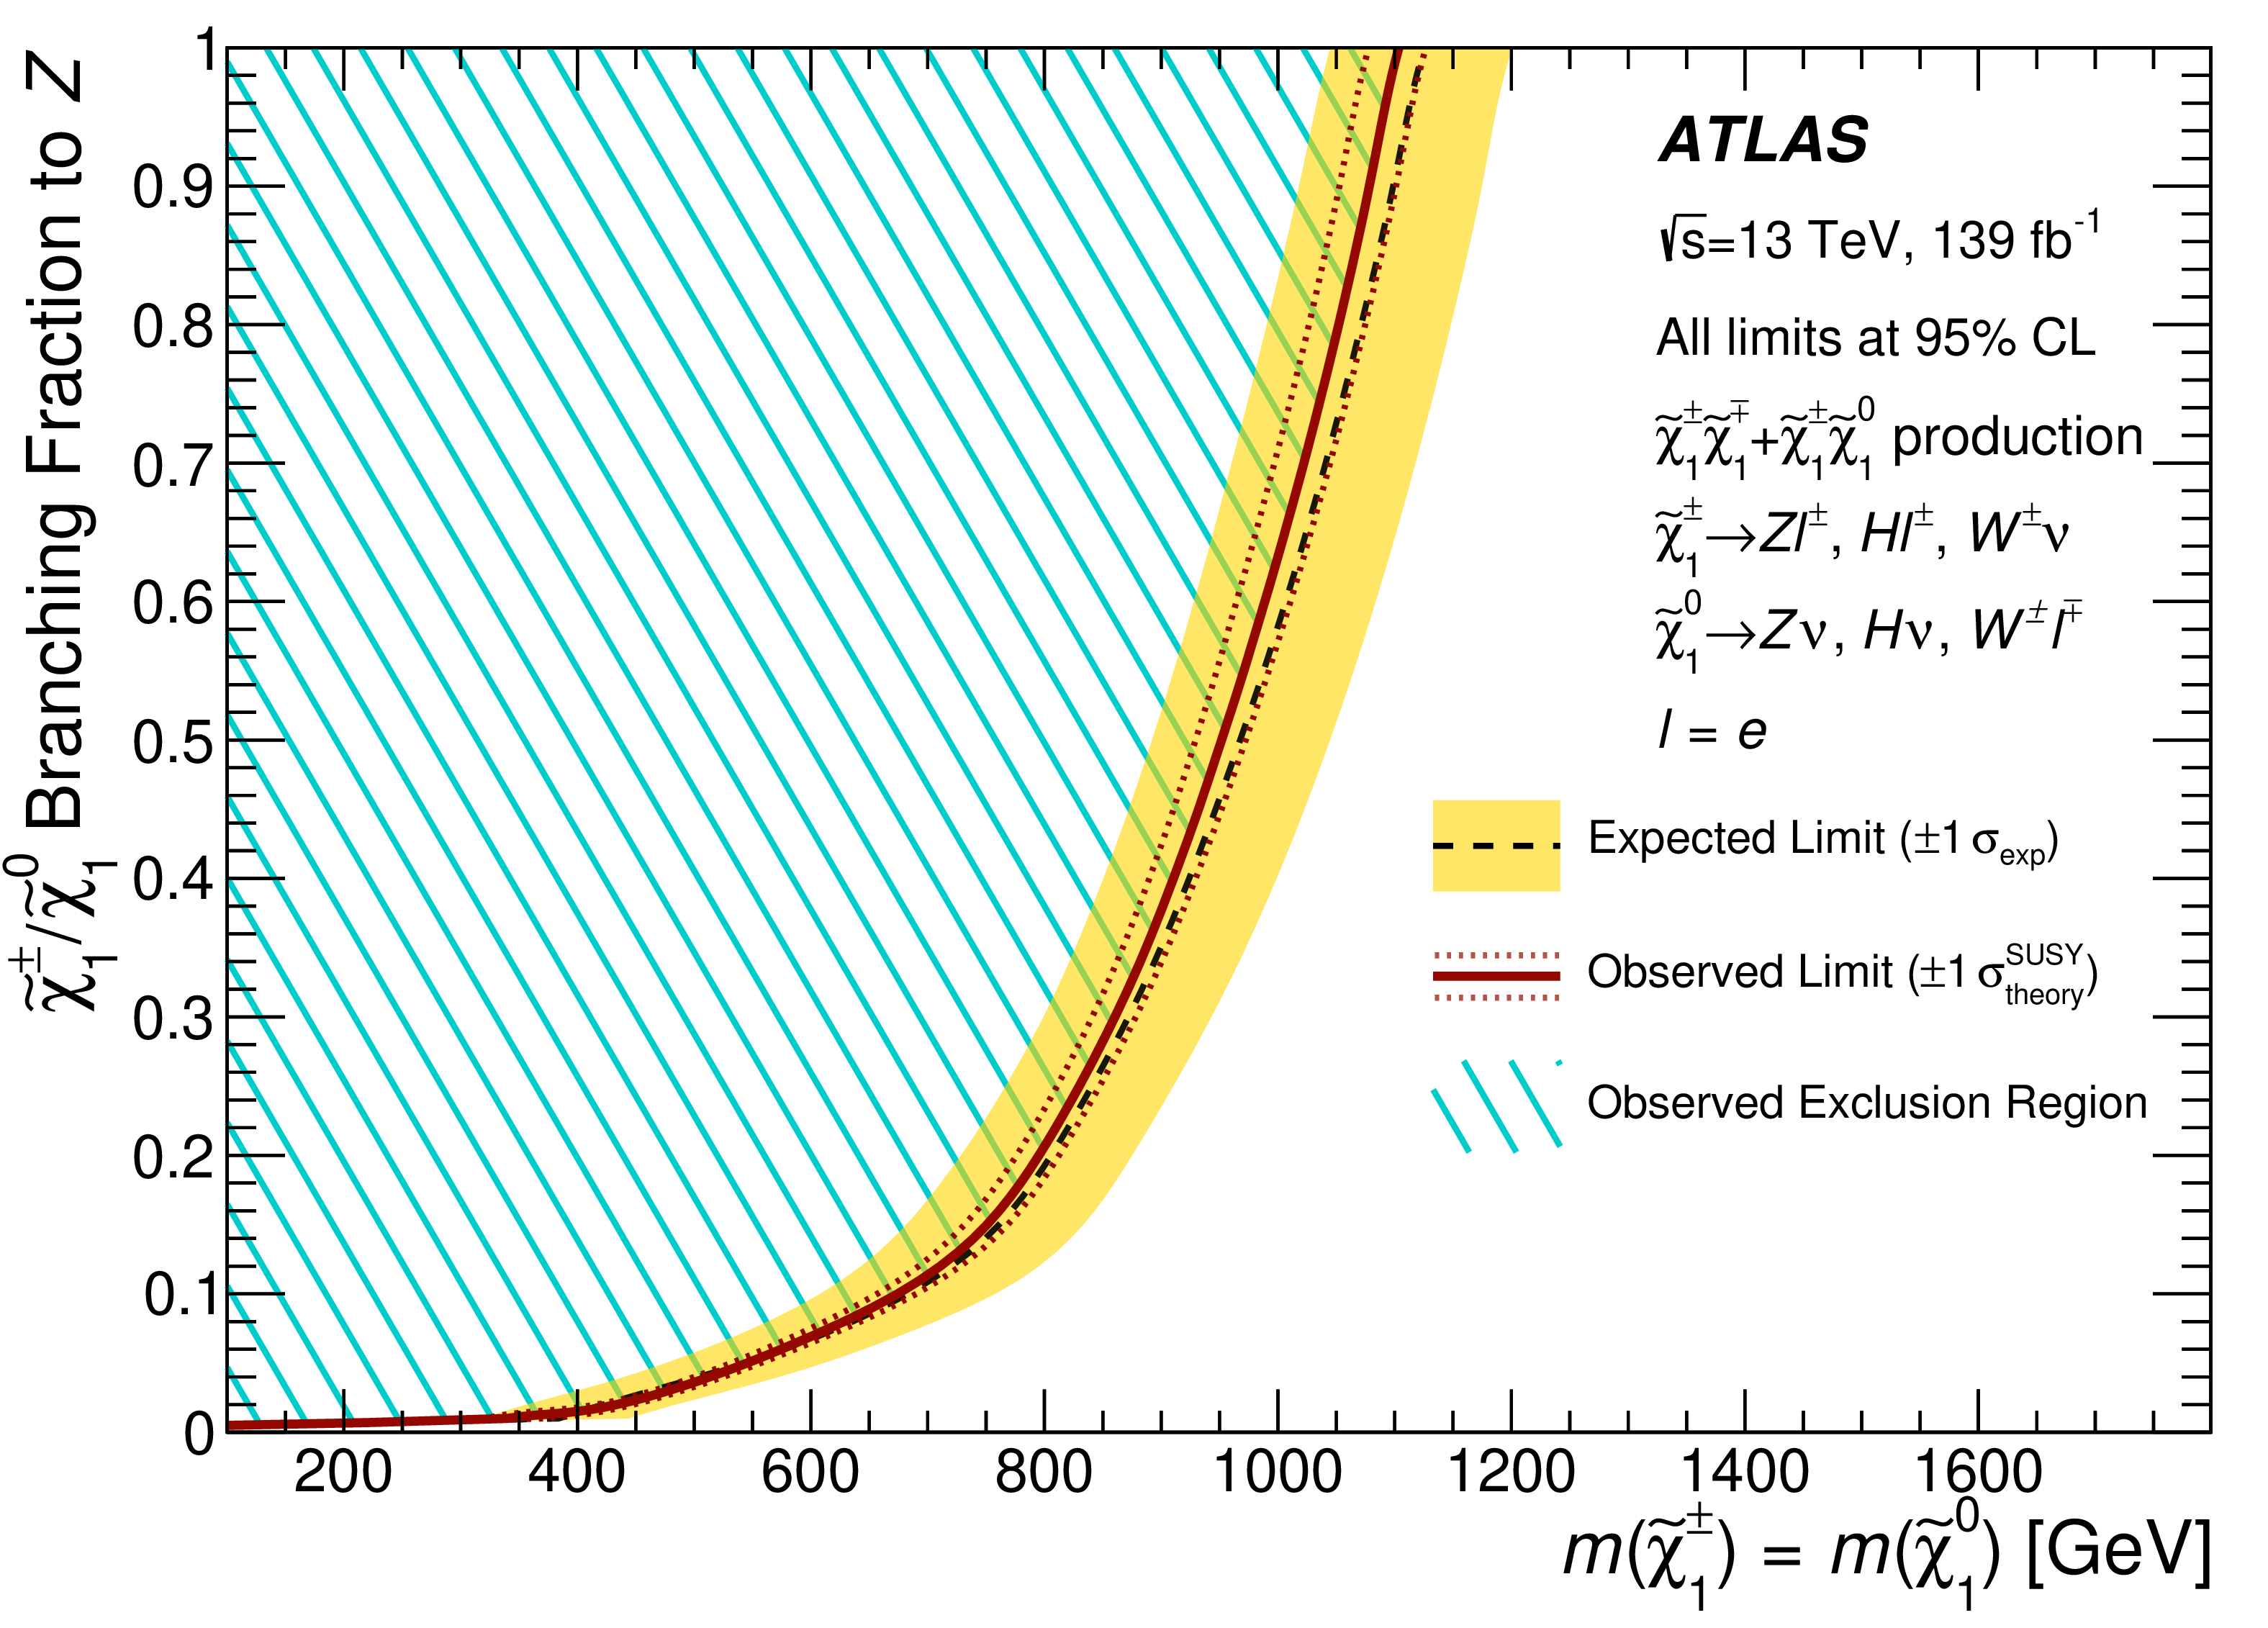
\includegraphics[width=0.98\textwidth]{figs/rpvthreel/contours_bre_100_brm_0_brt_0_Nominal.png}
      \caption{}
      \label{fig:contour_100e}
    \end{subfigure}
    \hfill
    \begin{subfigure}[b]{0.49\textwidth}
      \centering
      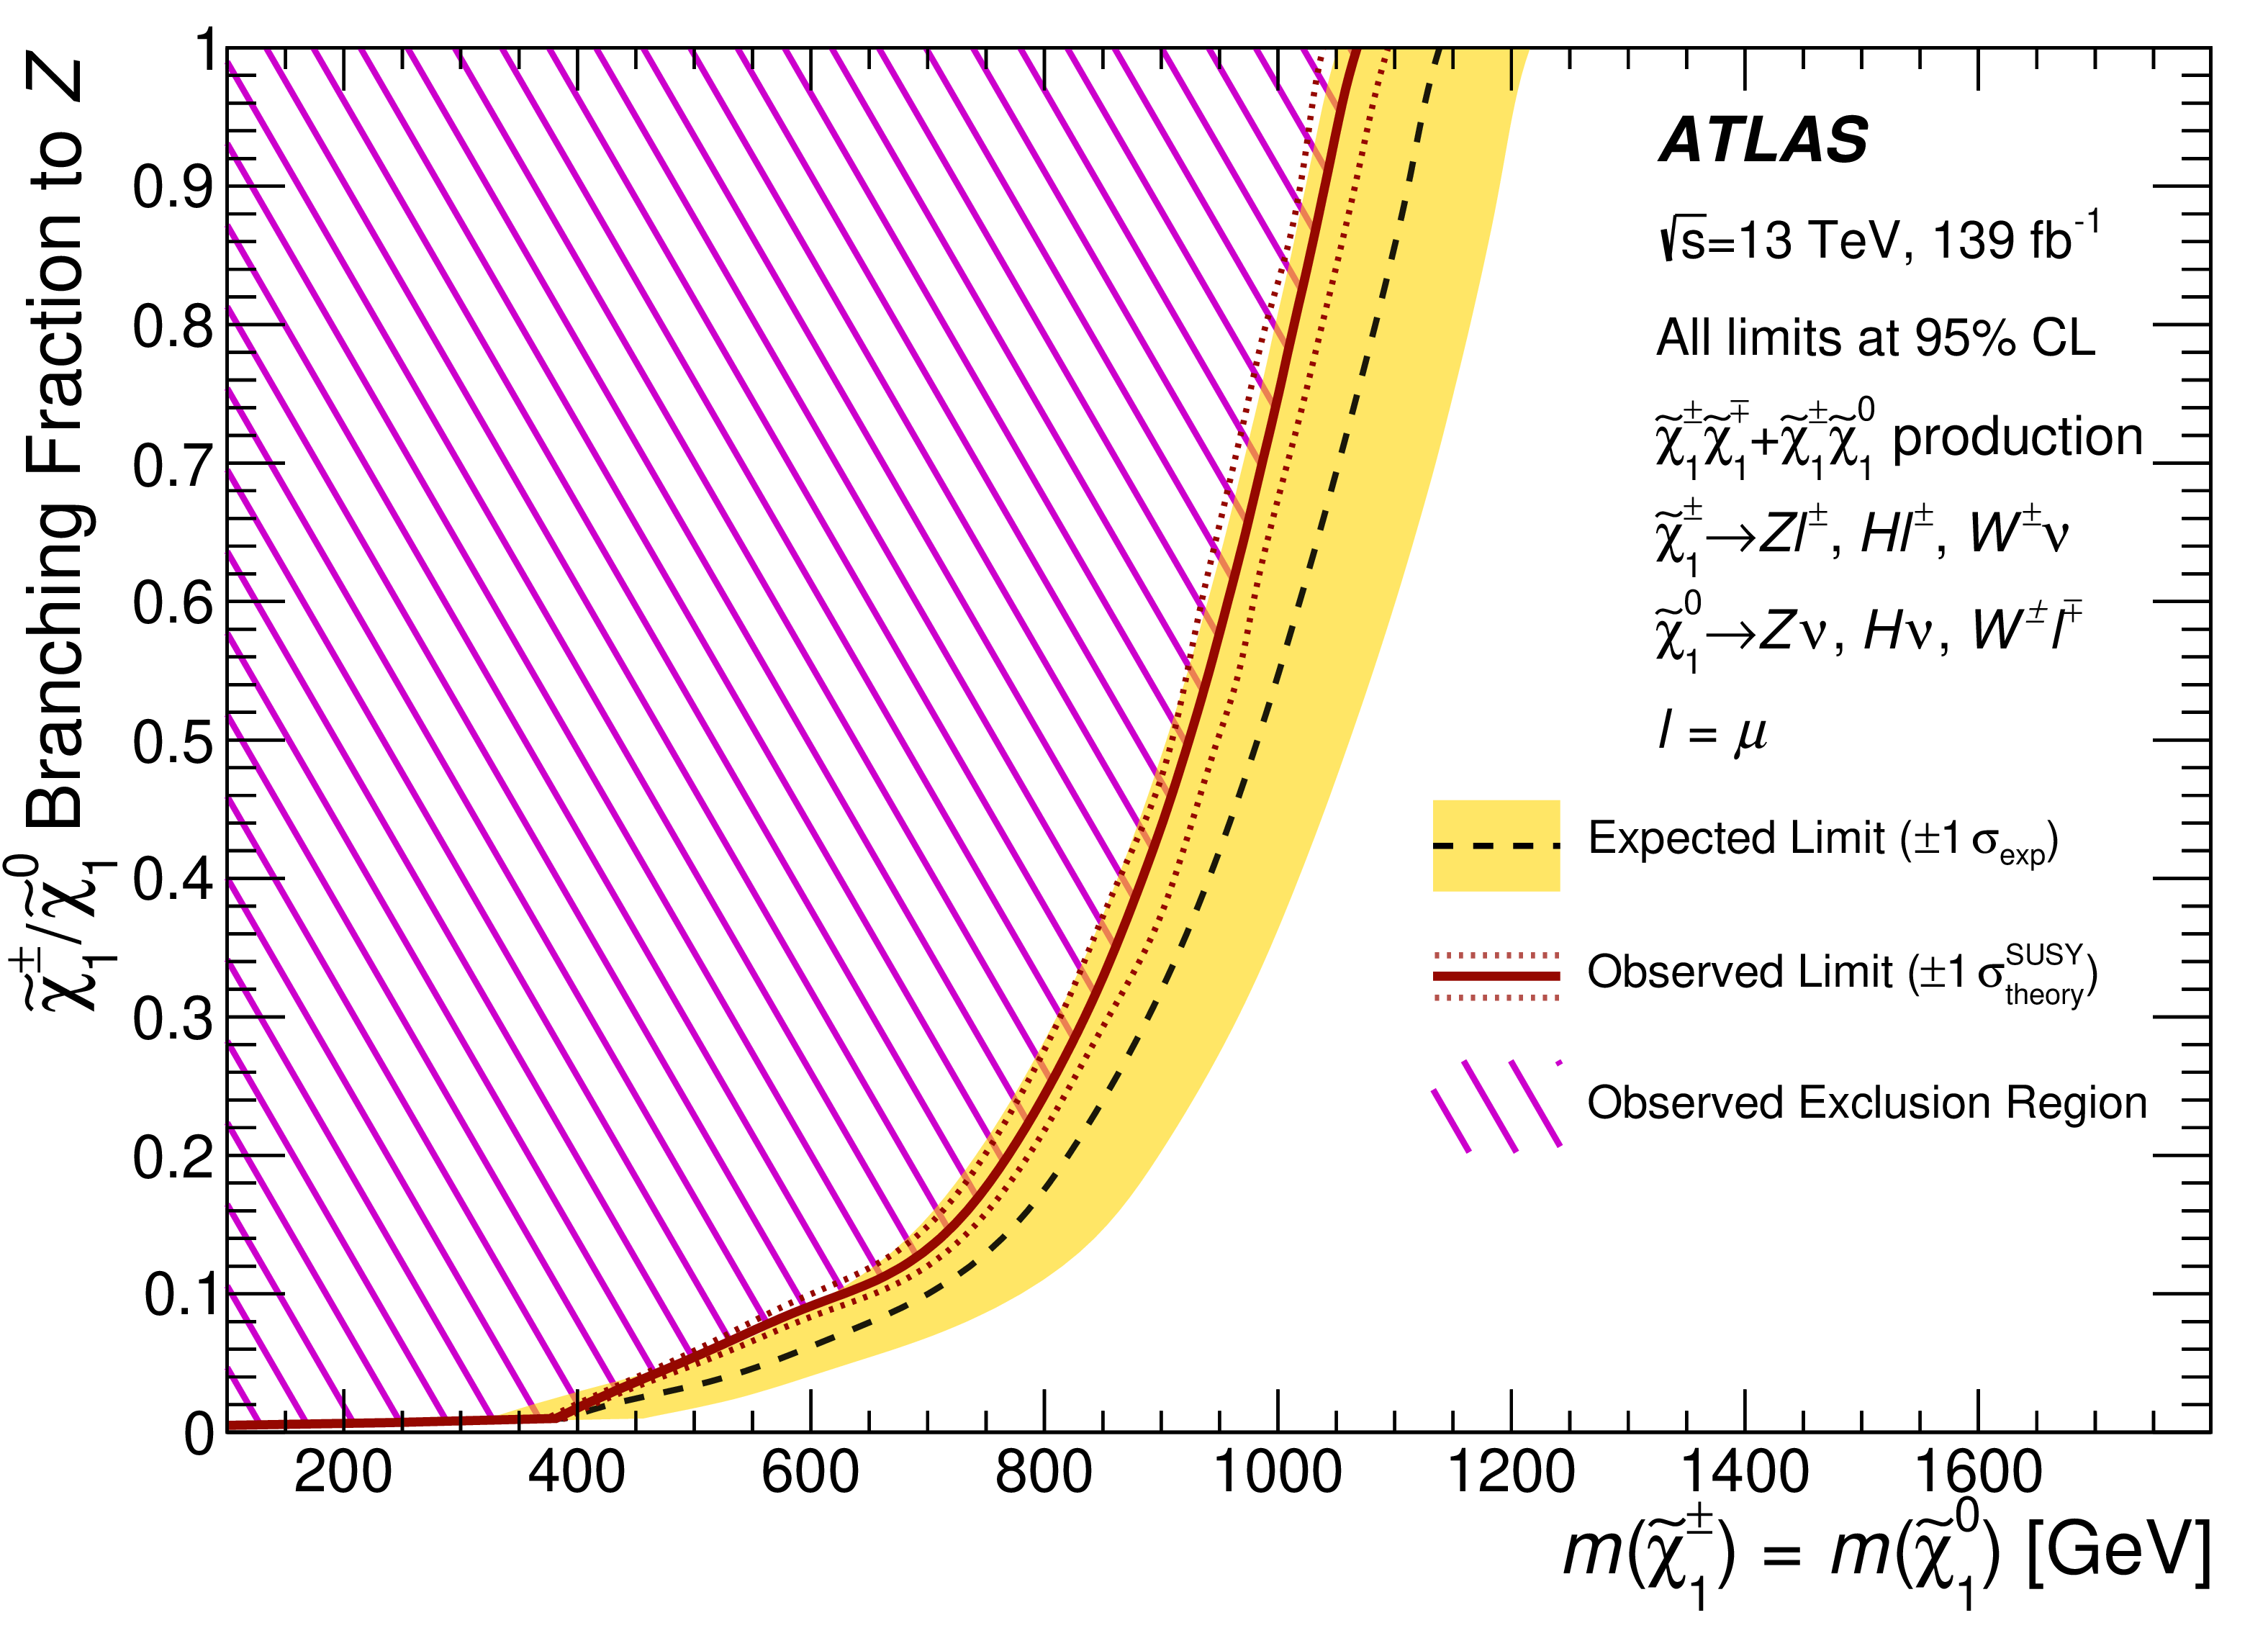
\includegraphics[width=0.98\textwidth]{figs/rpvthreel/contours_bre_0_brm_100_brt_0_Nominal.png}
      \caption{}
      \label{fig:contour_100mu}
    \end{subfigure}
    \begin{subfigure}[b]{0.49\textwidth}
      \centering
      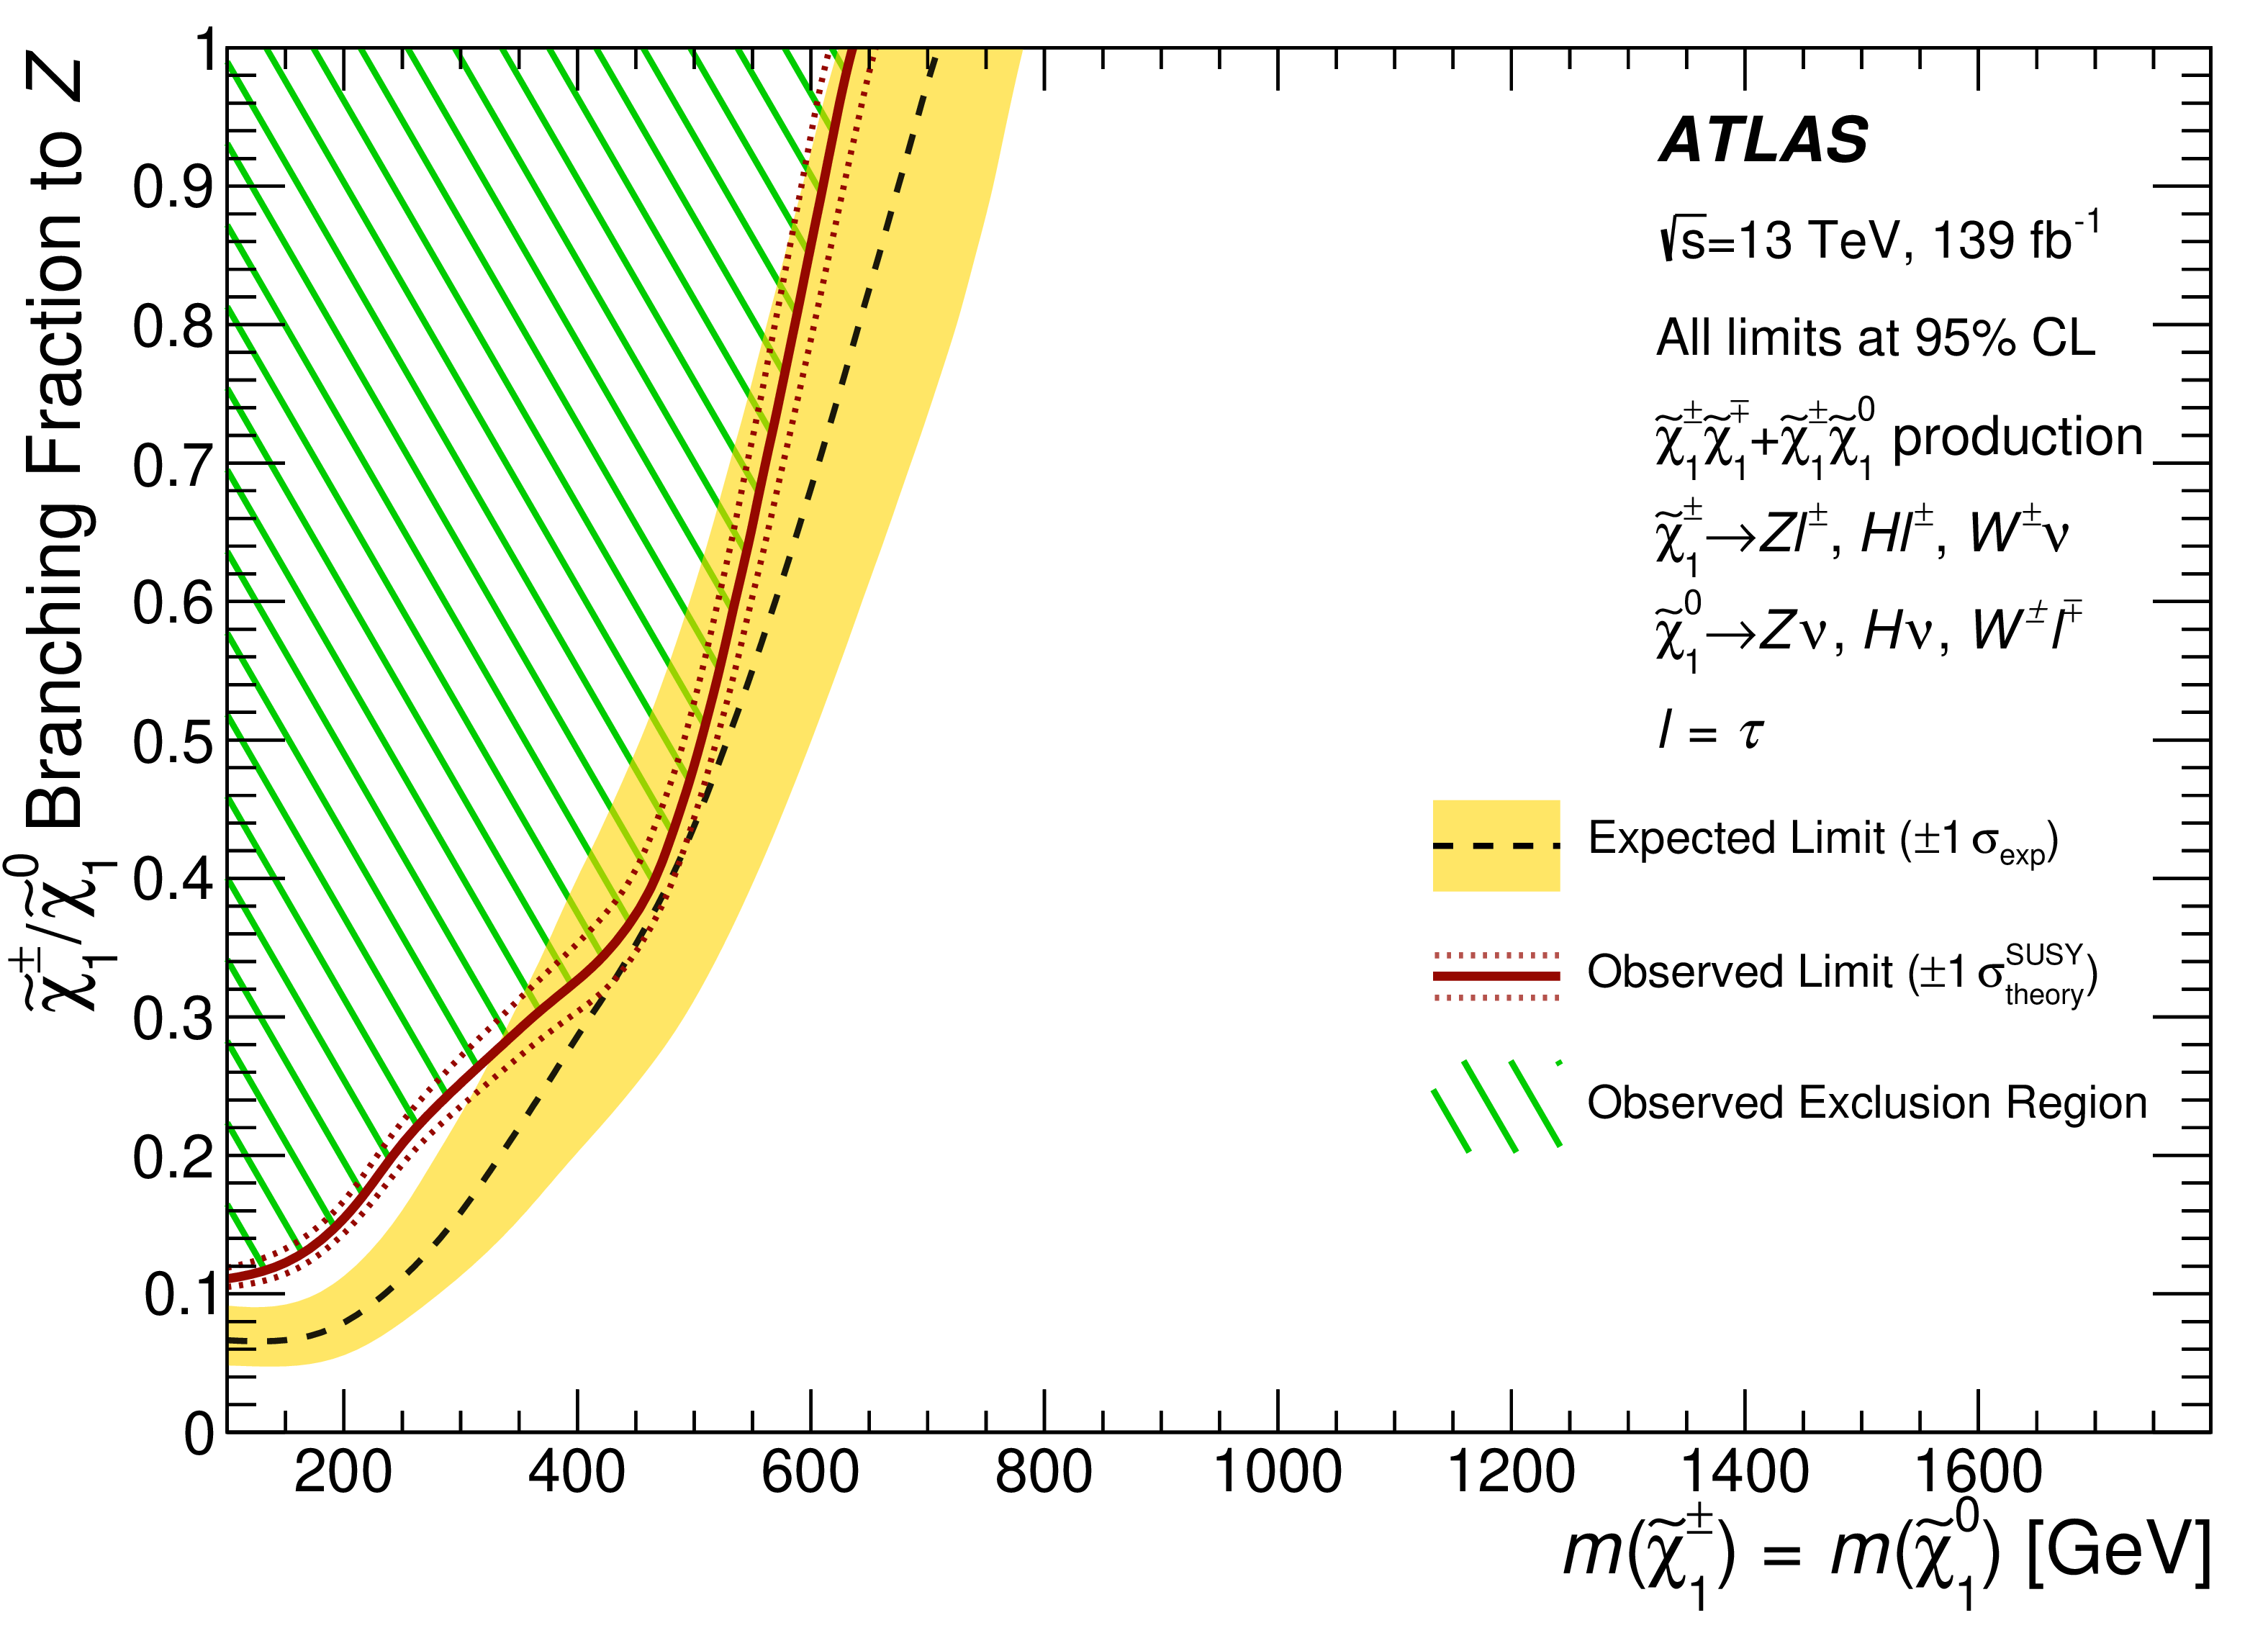
\includegraphics[width=0.98\textwidth]{figs/rpvthreel/contours_bre_0_brm_0_brt_100_Nominal.png}
      \caption{}
      \label{fig:contour_100tau}
    \end{subfigure}
    \caption[Exclusion curves for the simplified model of \CCsignal + \CNsignal production as a function of \chono mass and branching fraction to $Z$ bosons.]{Exclusion curves for the simplified model of \CCsignal + \CNsignal production as a function of \chono mass and branching fraction to $Z$ bosons.
    Curves are derived separately when requiring that the charged-lepton decays of \chono are into (a) any leptons with equal probability, (b) electrons only, (c) muons only, or (d) $\tau$-leptons only.
    \explimit
    \obslimit
    \exludedcolors
    The sum of the \chono branching fractions to $W$, $Z$, and Higgs bosons is unity for each point, and the branching fractions to $W$ and Higgs bosons are chosen so as to be equal everywhere~\cite{ATLAS:2020uer}.}
    \label{fig:contours}
\end{figure}

\subsection{Branching Ratio Limits on \BL production}
\label{sec:BRscan}
%\textcolor{red}{\hrulefill \textsc{Unfinished Section}\hrulefill}  \\
Since the charged and neutral winos in the \BL model have several possible decays, limits are set as a function of the wino branching ratio. 
Signal events are reweighted according to the truth decay of the wino to effectively set limits on each decay separately.
A scan is performed over each charged lepton flavor (electron, muon, and $\tau$-lepton) and over each possible boson type (\(Z,W,\) and higgs). 
The considered points in the lepton flavor scan are (BR(\wino$\rightarrow$ \(Be\)), BR(\wino$\rightarrow$ \(B\mu\)), BR(\wino$\rightarrow$ \(B\tau\)))=(1, 0, 0), (0, 1, 0), (0, 0, 1), and (0.33, 0.33, 0.33), where \(B\) is a W boson for the \none scan, and can be either a \Zboson\ or a Higgs for the \chone scan.
Then for each of these points, a finer granularity scan is performed over the possible boson types of the wino decay, steps of 10\% for BR to \Zboson\ and 20\% for BR to \Hboson. 
Limits are set as a function of BR(\chone$\rightarrow H\ell$) vs BR(\chone$\rightarrow Z\ell$) for \chone and BR(\none $\rightarrow H\nu$) vs BR(\none$\rightarrow Z\nu$) for \none, separately for each considered wino-to-lepton branching ratio point.
The BR(\chone$\rightarrow W\nu$) and  BR(\none$\rightarrow W\ell$) are implicitly included on the respective 2D plots since the sum of the three BRs must equal 1.
%The \mZl distributions achieved from three example boson BR points (brZ=100\%, brZ=10\% and brH=90\%, and brZ=10\% and brW=90\%) are shown in \appref{BRreweightingExamples}, for all three SRs.
To increase sensitivity for the BR(\wino$\rightarrow$ \(Be\))=100\% and BR(\wino$\rightarrow$ \(B\mu\))=100\% scenarios in the lepton flavor scan, additional SR selections are applied on the flavor of the third lepton which is assumed to come directly from the \chone or \none decay (that which is assigned to the \Zl leg but not assigned to the Z). 
For BR(\wino$\rightarrow$ \(Be\))=100\% limits, this lepton is required to be an electron, and for BR(\wino$\rightarrow$ \(B\mu\))=100\% limits, this lepton is required to be a muon.
\SRFR events require that all leptons assigned directly to the \chone or \none decay (and not to a boson) must have the required flavor.
This imposes the requirement that both winos decay to the same lepton flavor, as predicted in the \BL model because the wino-to-lepton BR is dictated by the neutrino hierarchy and hence should be the same for charginos and neutralinos.
\SRFour events are agnostic to the fourth lepton flavor. 
The reasoning for this, as opposed to the agreement between the third and fourth leptons which is required in \SRFR, is because in \SRFour the fourth lepton can often come from the second boson decay and hence its flavor is random compared to the lepton directly from the wino decay.
The other two points in the lepton flavor scan (fully tau and flavor democratic) allow all lepton flavors.
%The expected yields and \mZl distributions for these additional SR criteria are shown in \appref{lepFlavorSRs}.
Limits are set simultaneously for \CCsignal and \CNsignal production modes.
This effectively imposes the assumption that the \chone and \none decay BRs are fully correlated, for both lepton and boson decays.
%Limits are shown in Figures \ref{fig:triangles} for the 600~\GeV mass point.
Figures \ref{fig:contour_democratic} to \ref{fig:contour_100tau} show limits set in the plane of \chono branching fraction to the \Zboson\ boson vs the \chono mass, for each of the lepton flavor scenarios. 
The strongest exclusions come from BR(\wino$\rightarrow$\(Be\))=100\% and BR(\wino$\rightarrow$\(B\mu\))=100\% points in the scan as expected as light flavor leptons were only targeted in this analysis, sensitivity to the BR(\wino$\rightarrow$\(B\tau\))=100\% point comes from leptonic tau decays.  
Figures \ref{fig:triangle_democratic} to \ref{fig:triangle_100tau} show the limits set for the hypothesis of a \chono with a mass of 600~\GeV to show the limits in the plane of the \chono branching fraction to Higgs vs \Zboson.  
The vertical nature of the limits shows the strong dependence (as expected) on the \Zboson\ boson branching fraction and little dependence on the Higgs or \Wboson\ boson branching fraction.
\begin{figure}[ht]
    \centering
    \begin{subfigure}[b]{0.49\textwidth}
      \centering
      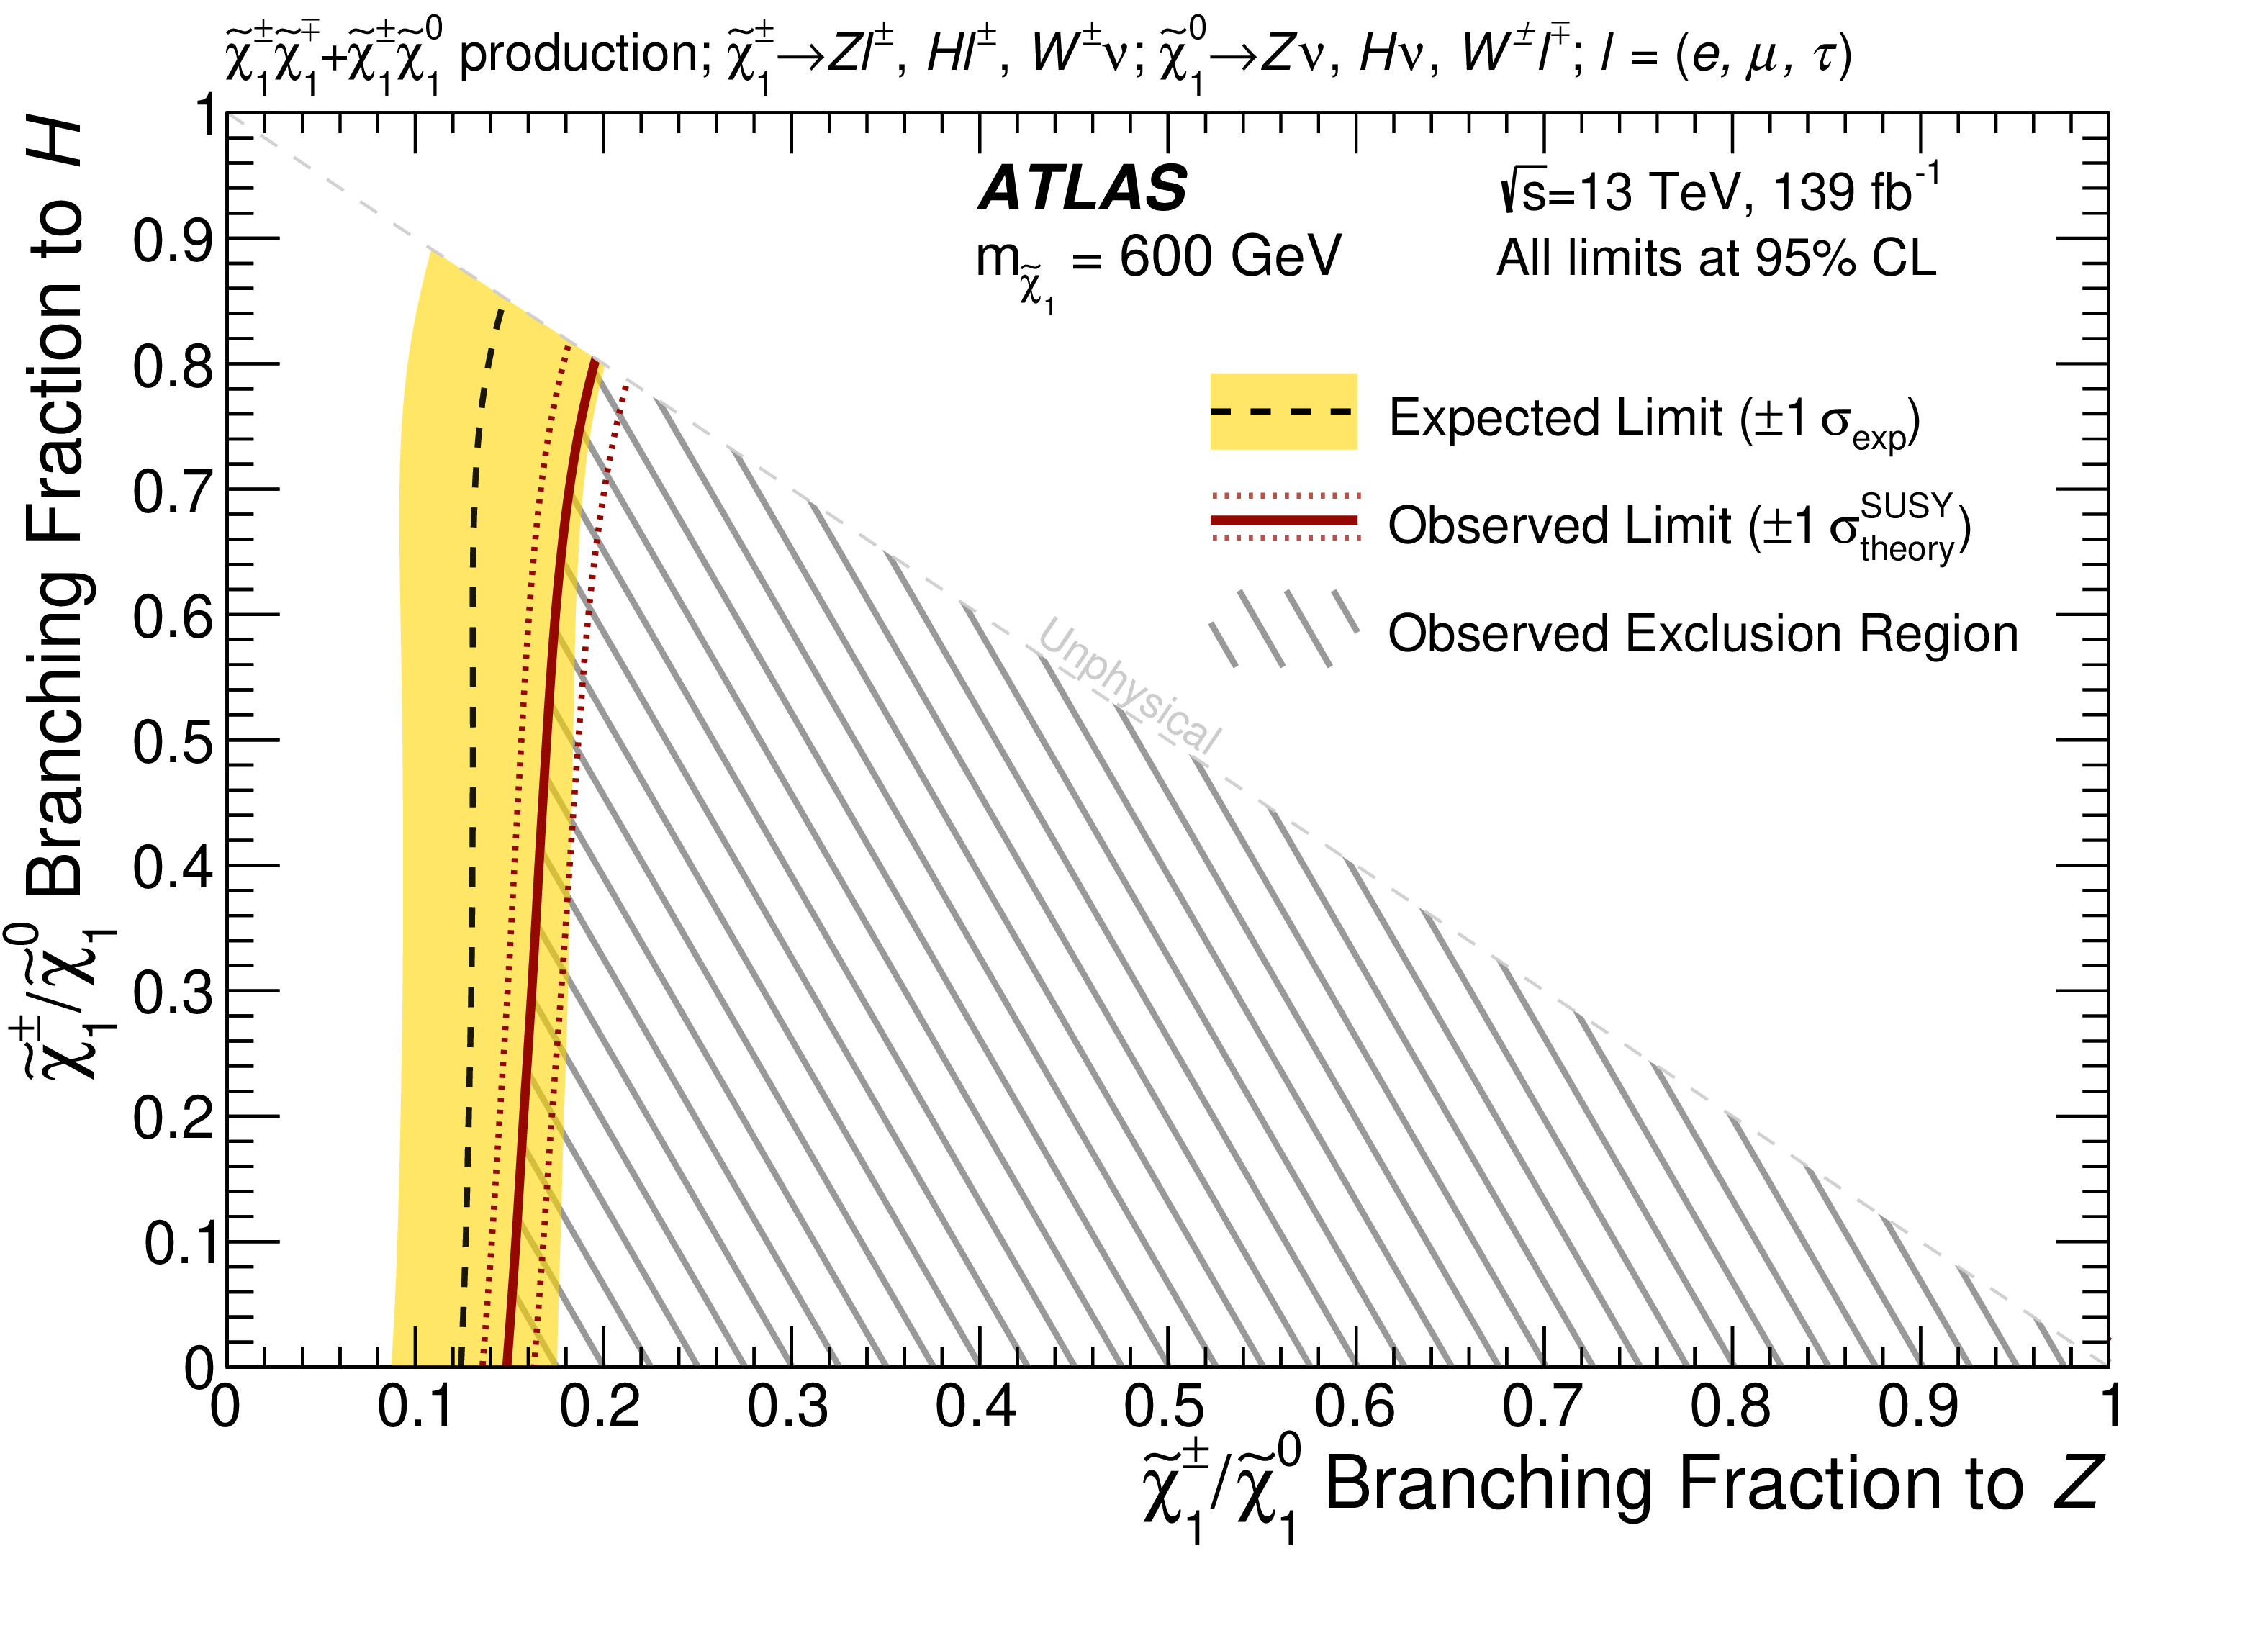
\includegraphics[width=0.98\textwidth]{figs/rpvthreel/triangleLimits_bre_33_brm_33_brt_33_mass_600.png}
      \caption{}
      \label{fig:triangle_democratic}
    \end{subfigure}
    \hfill
    \begin{subfigure}[b]{0.49\textwidth}
      \centering
      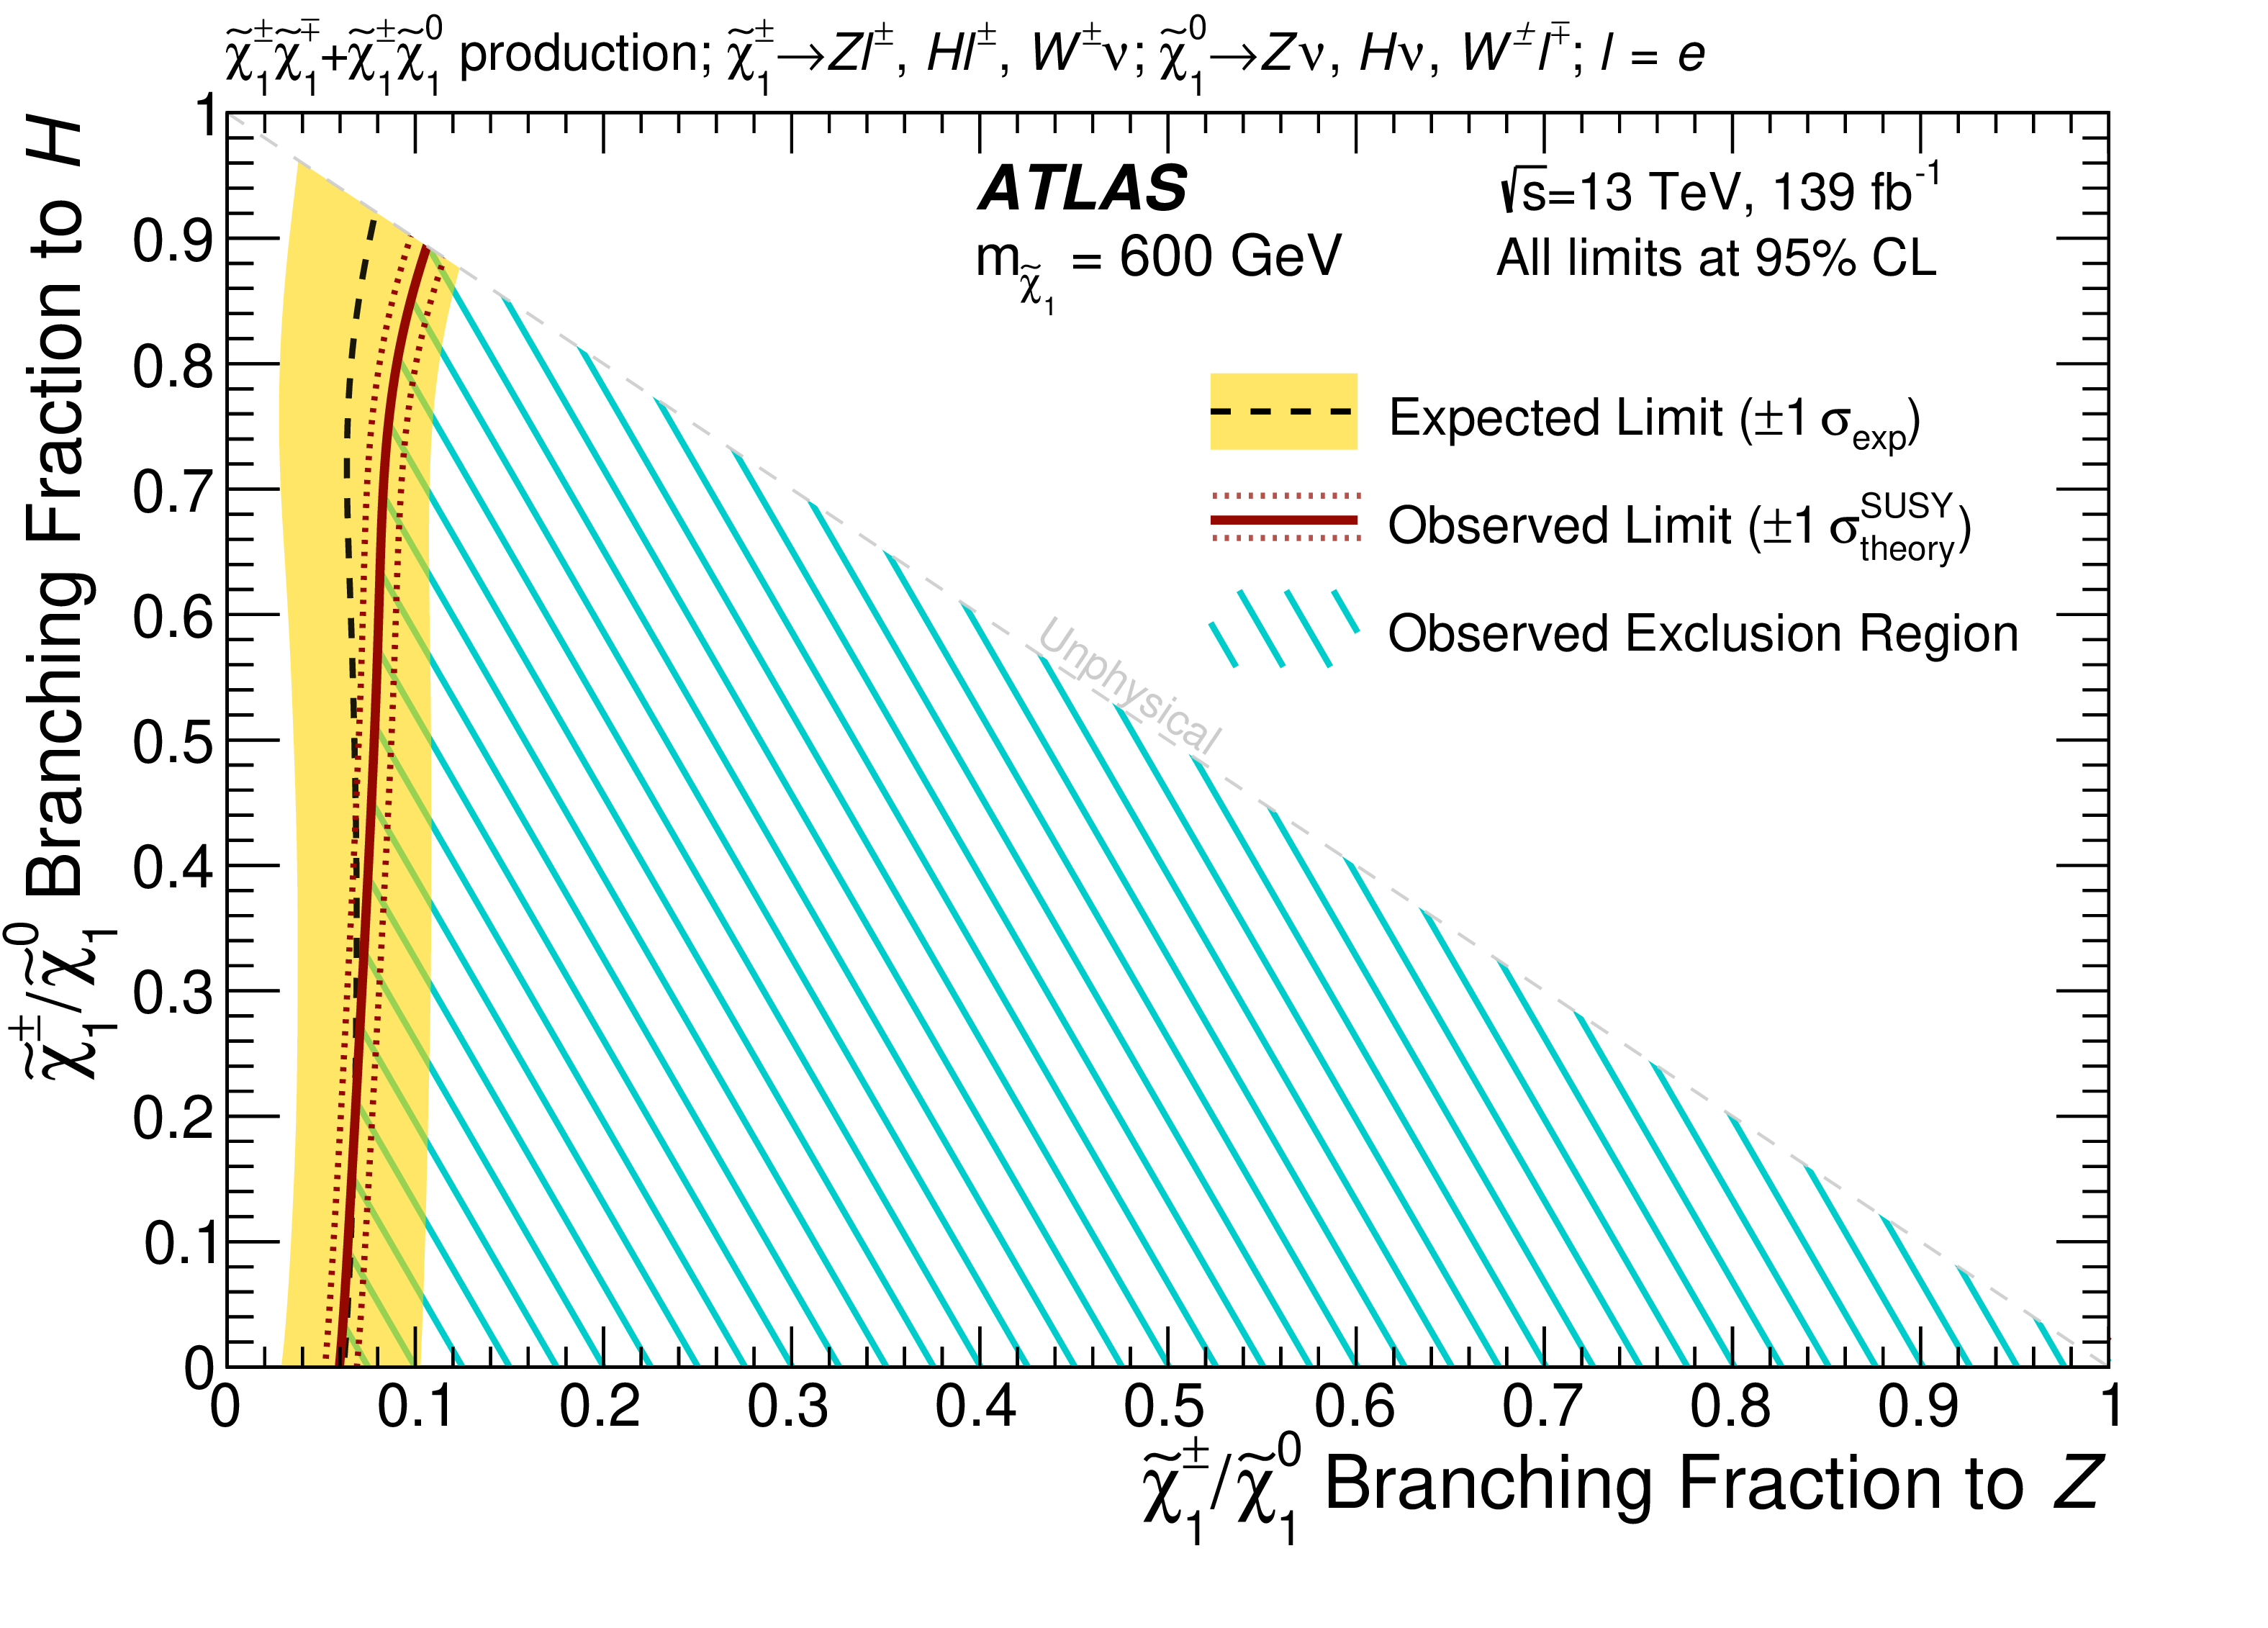
\includegraphics[width=0.98\textwidth]{figs/rpvthreel/triangleLimits_bre_100_brm_0_brt_0_mass_600.png}
      \caption{}
      \label{fig:trianlge_100e}
    \end{subfigure}
    \hfill
    \begin{subfigure}[b]{0.49\textwidth}
      \centering
      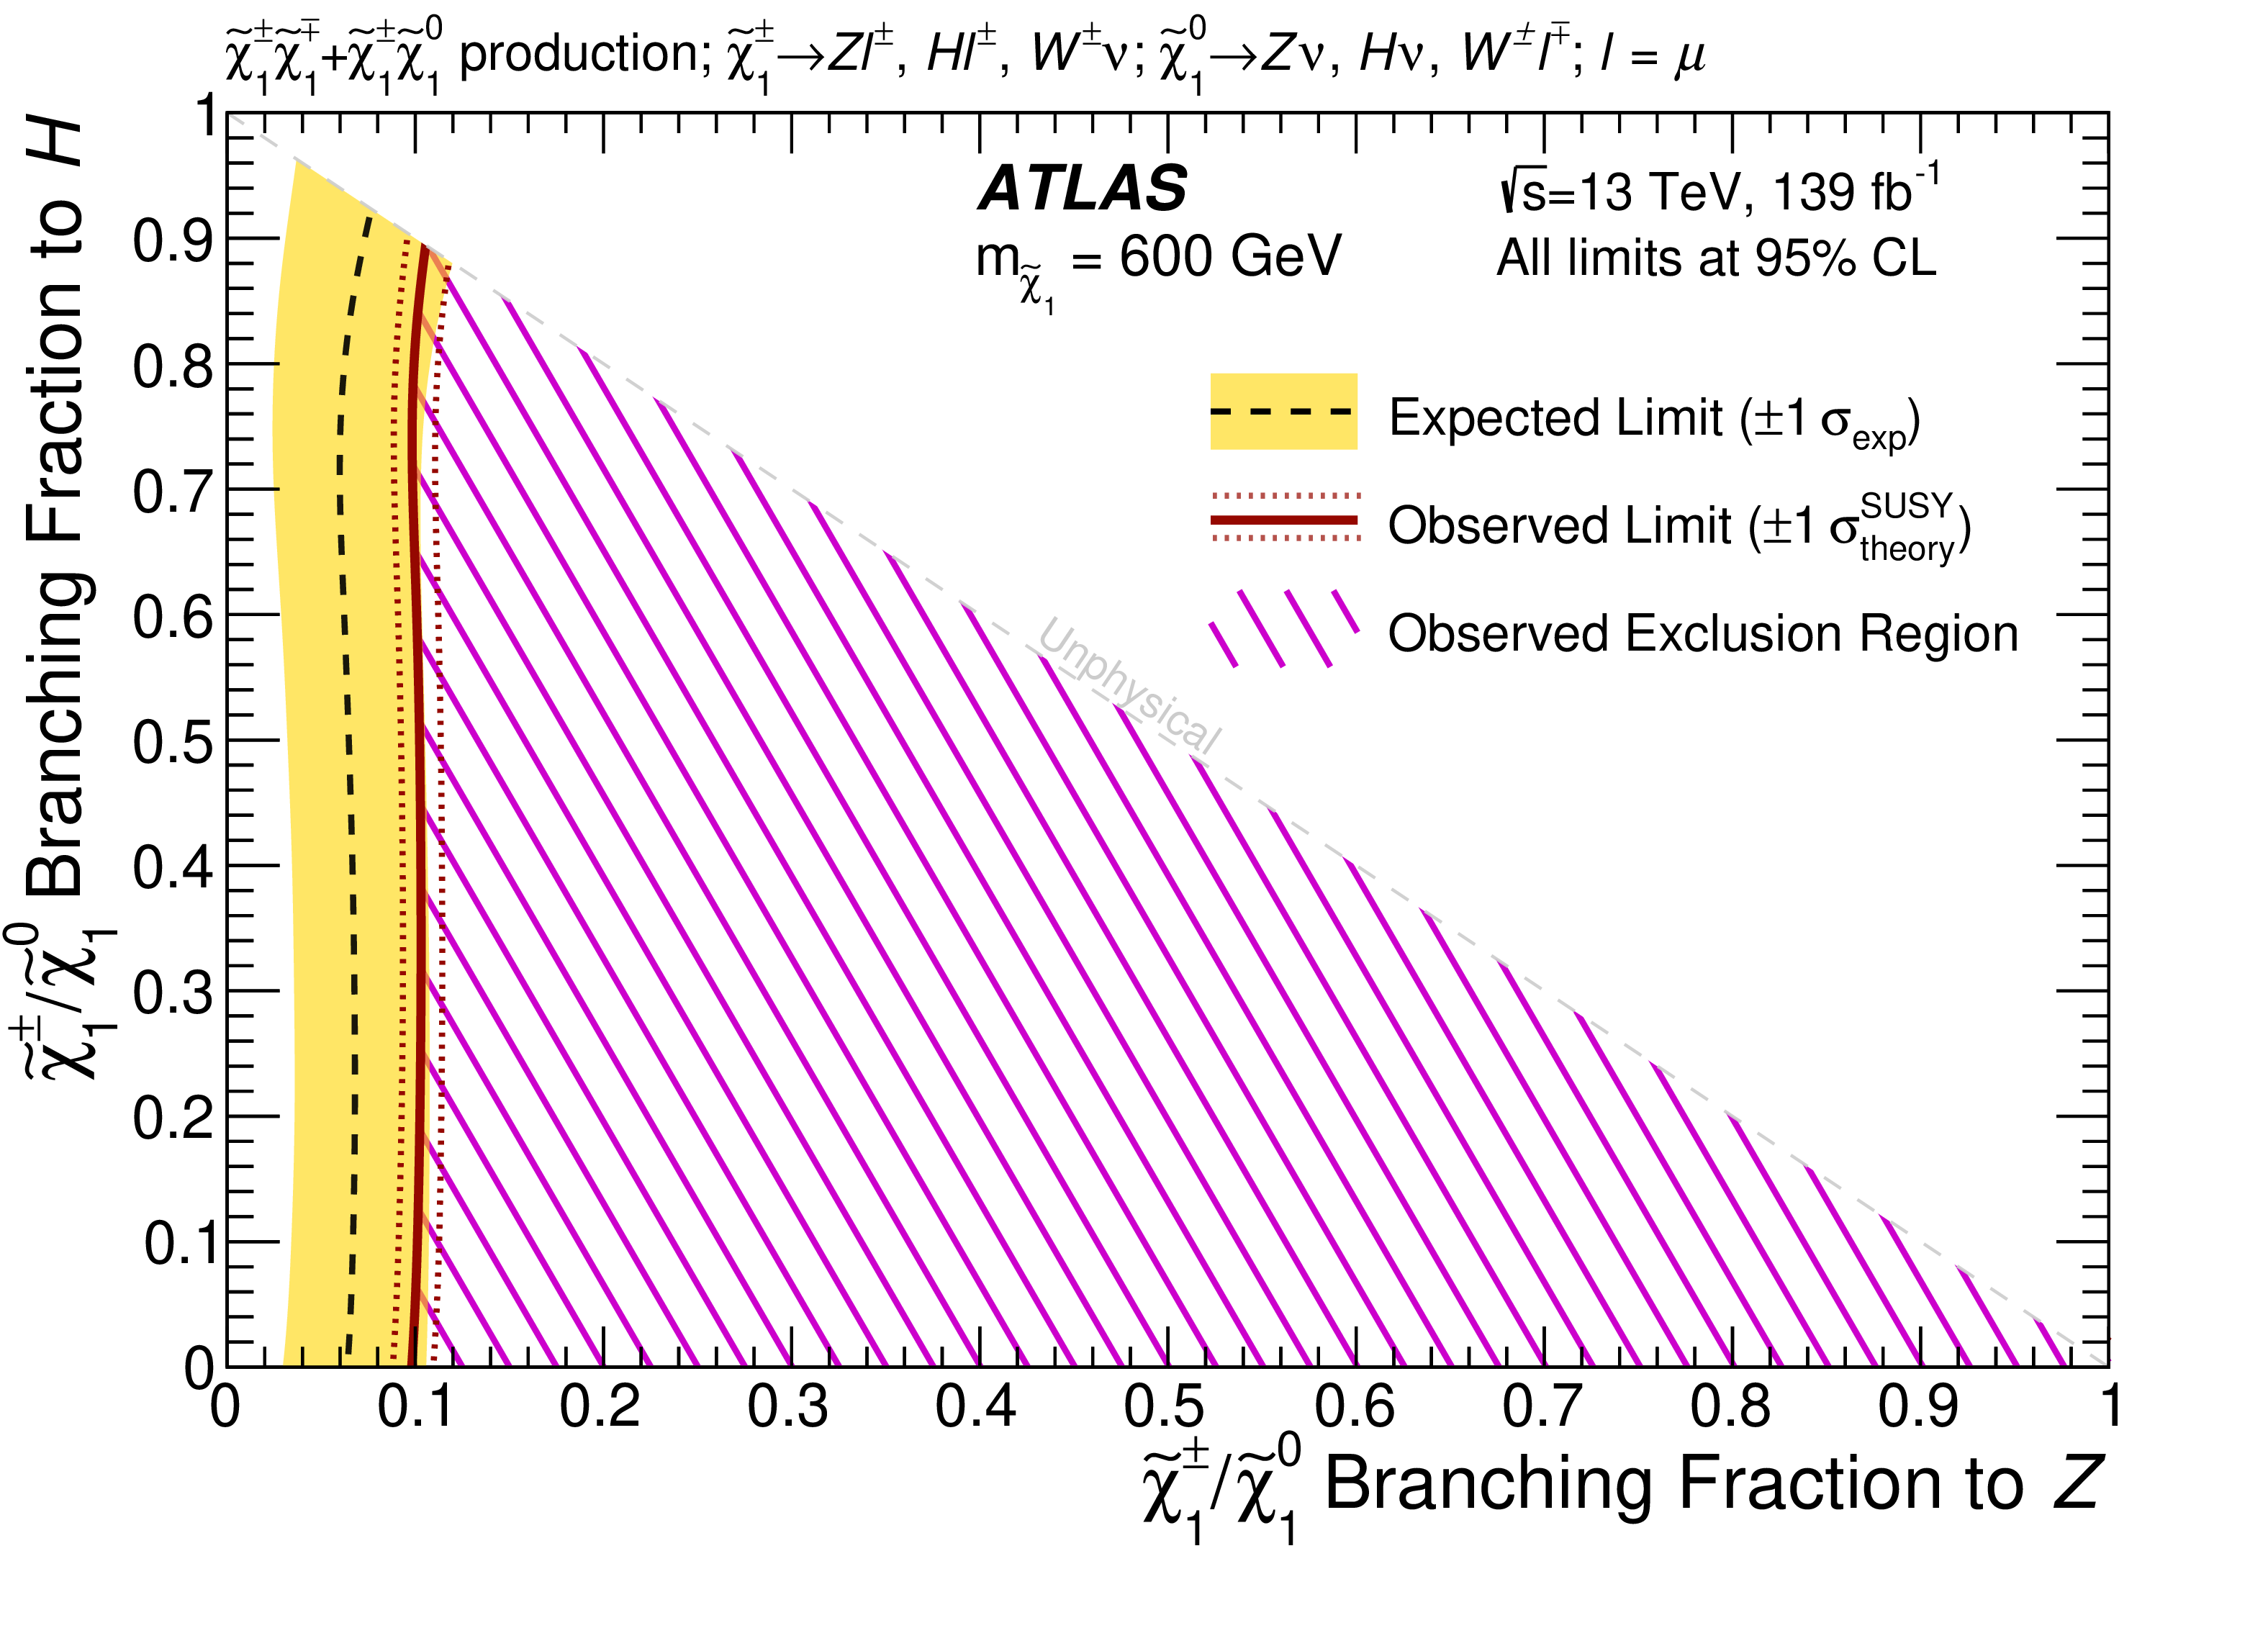
\includegraphics[width=0.98\textwidth]{figs/rpvthreel/triangleLimits_bre_0_brm_100_brt_0_mass_600.png}
      \caption{}
      \label{fig:triangle_100mu}
    \end{subfigure}
    \begin{subfigure}[b]{0.49\textwidth}
      \centering
      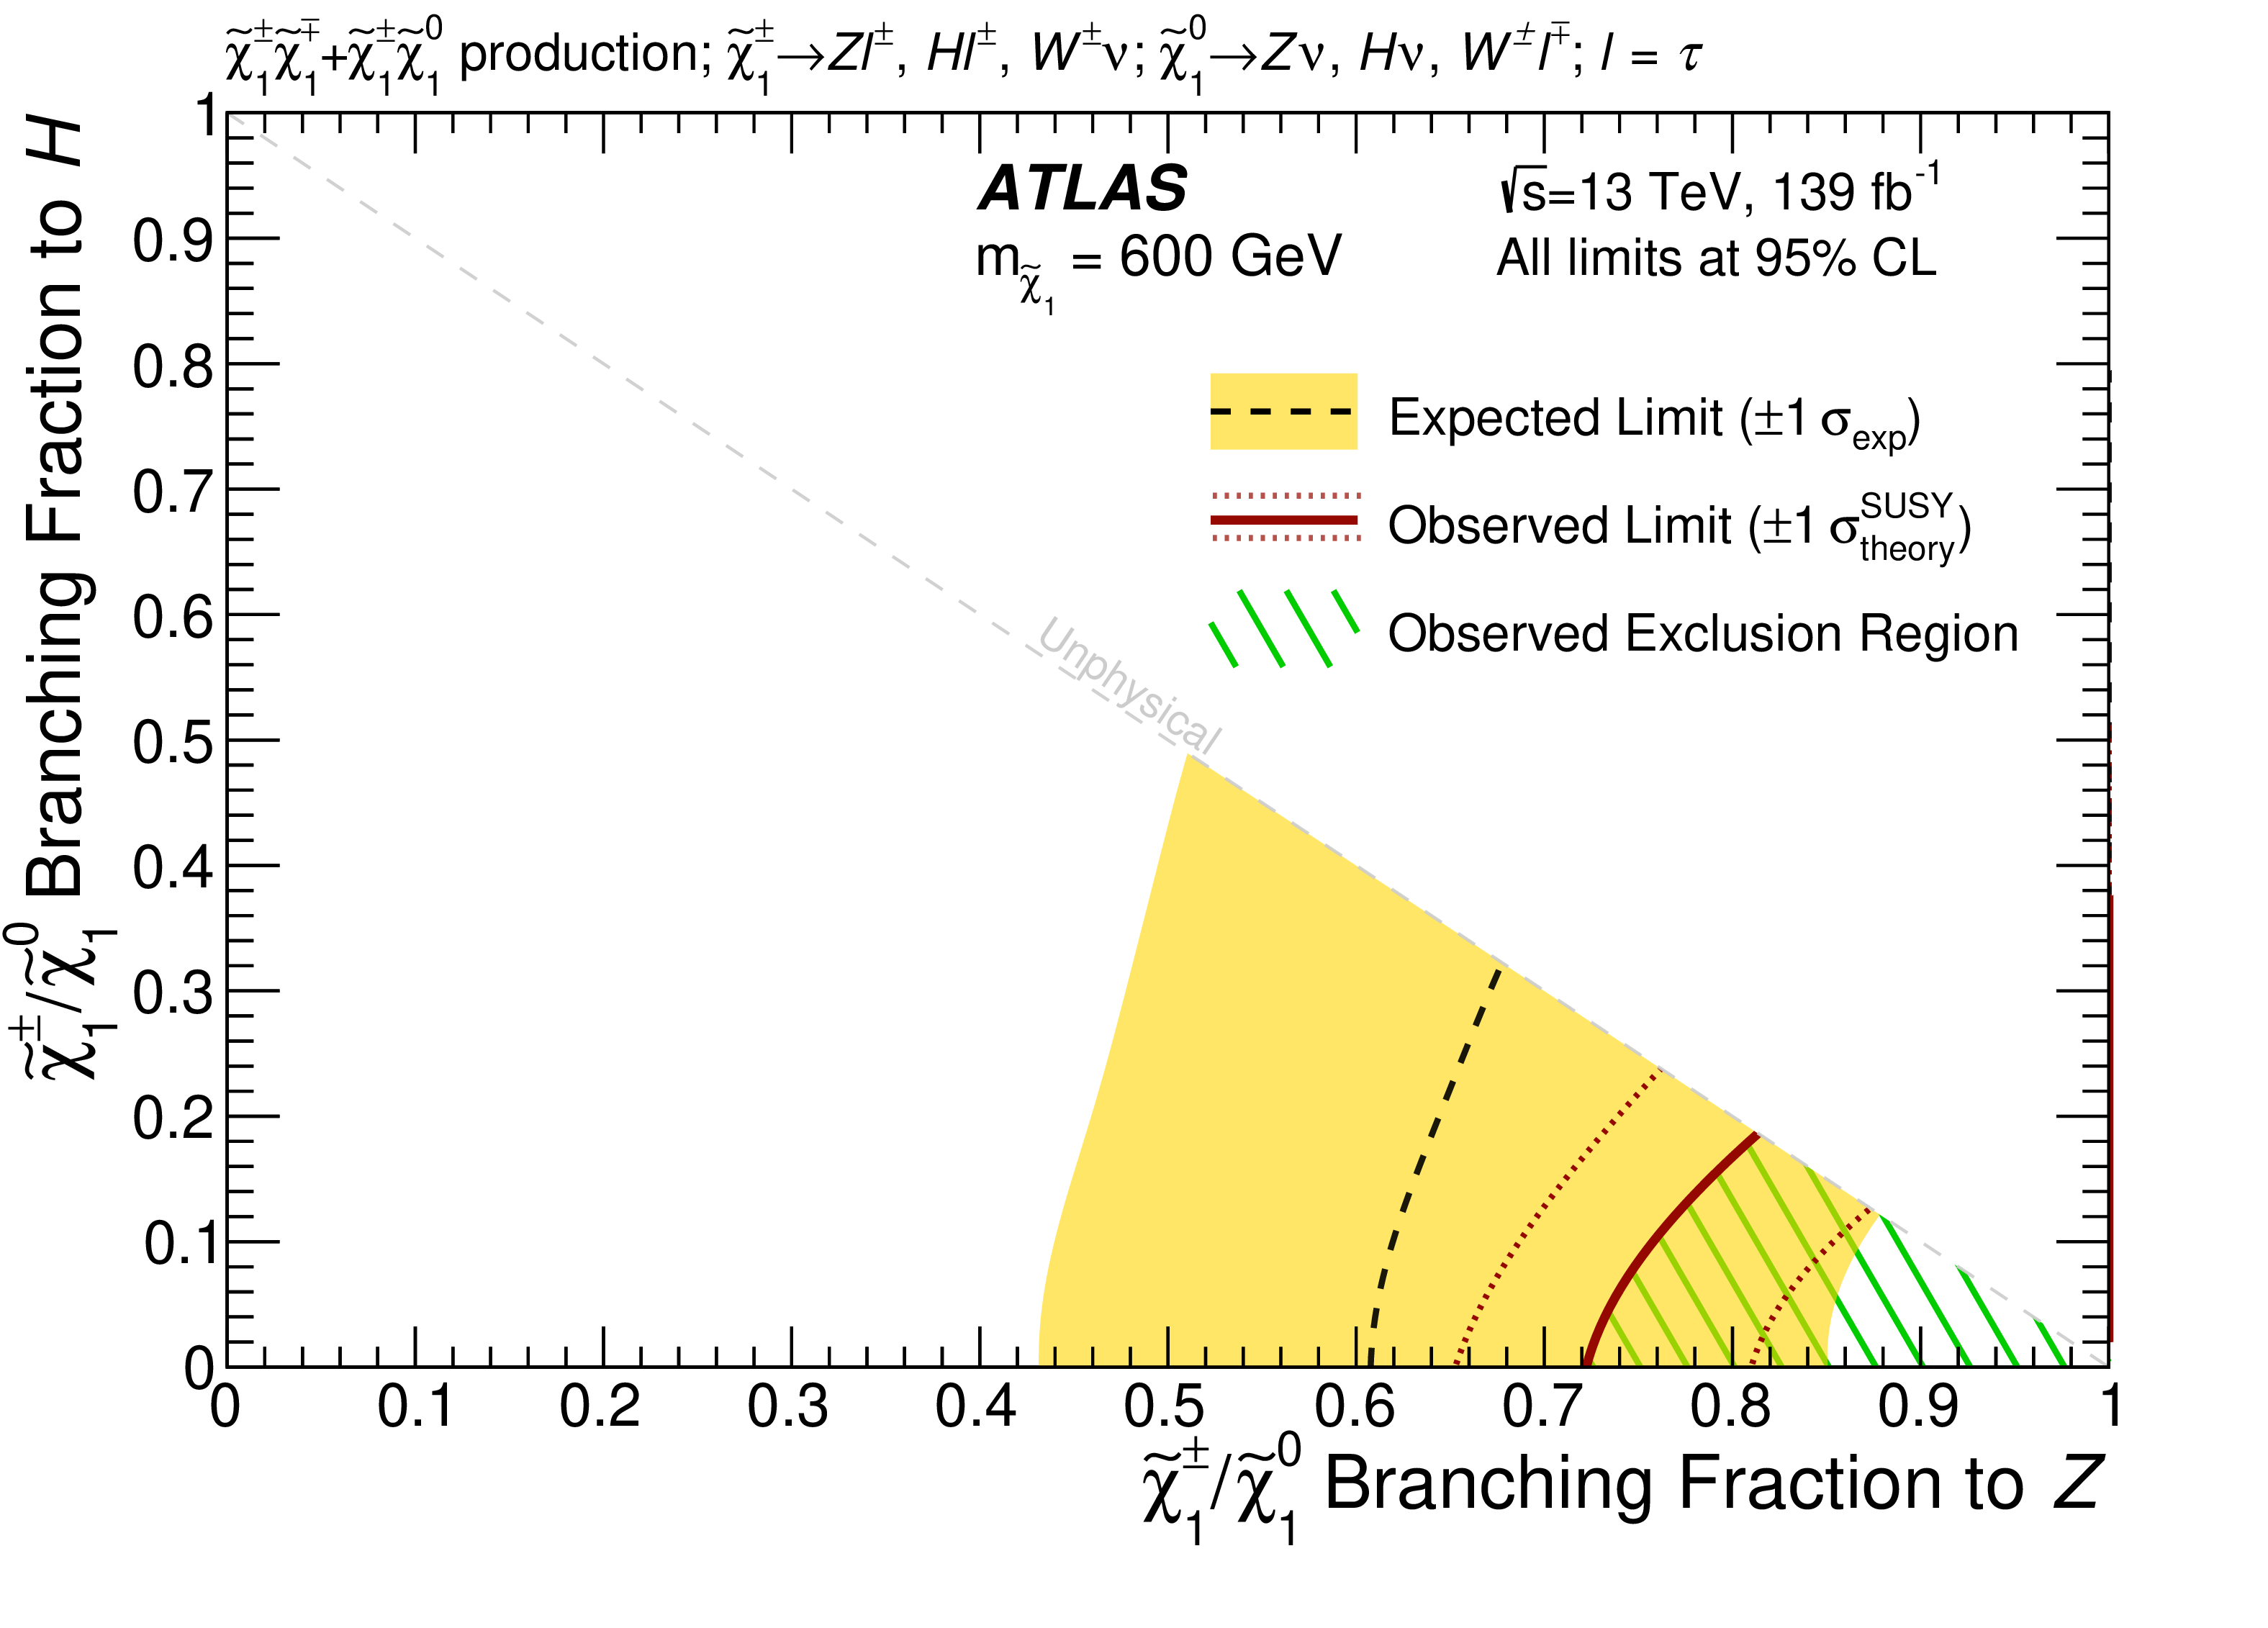
\includegraphics[width=0.98\textwidth]{figs/rpvthreel/triangleLimits_bre_0_brm_0_brt_100_mass_600.png}
      \caption{}
      \label{fig:triangle_100tau}
    \end{subfigure}
    \caption[Exclusion curves for the simplified model of \CCsignal + \CNsignal production as a function of the branching fractions to $Z$ and Higgs bosons.]{Exclusion curves for the simplified model of \CCsignal + \CNsignal production as a function of the branching fractions to $Z$ and Higgs bosons.
    Results are shown for the charged-lepton decays of \chono into (a) any leptons with equal probability, (b) electrons only, (c) muons only, and (d) $\tau$-leptons only for the 600~\GeV mass point. 
    \explimit
    \obslimit
    \exludedcolors
    \cite{ATLAS:2020uer}.}
    \label{fig:triangles}
\end{figure}
%\begin{figure}[ht]
%    \centering
%    \begin{subfigure}[b]{0.49\textwidth}
%      \centering
%      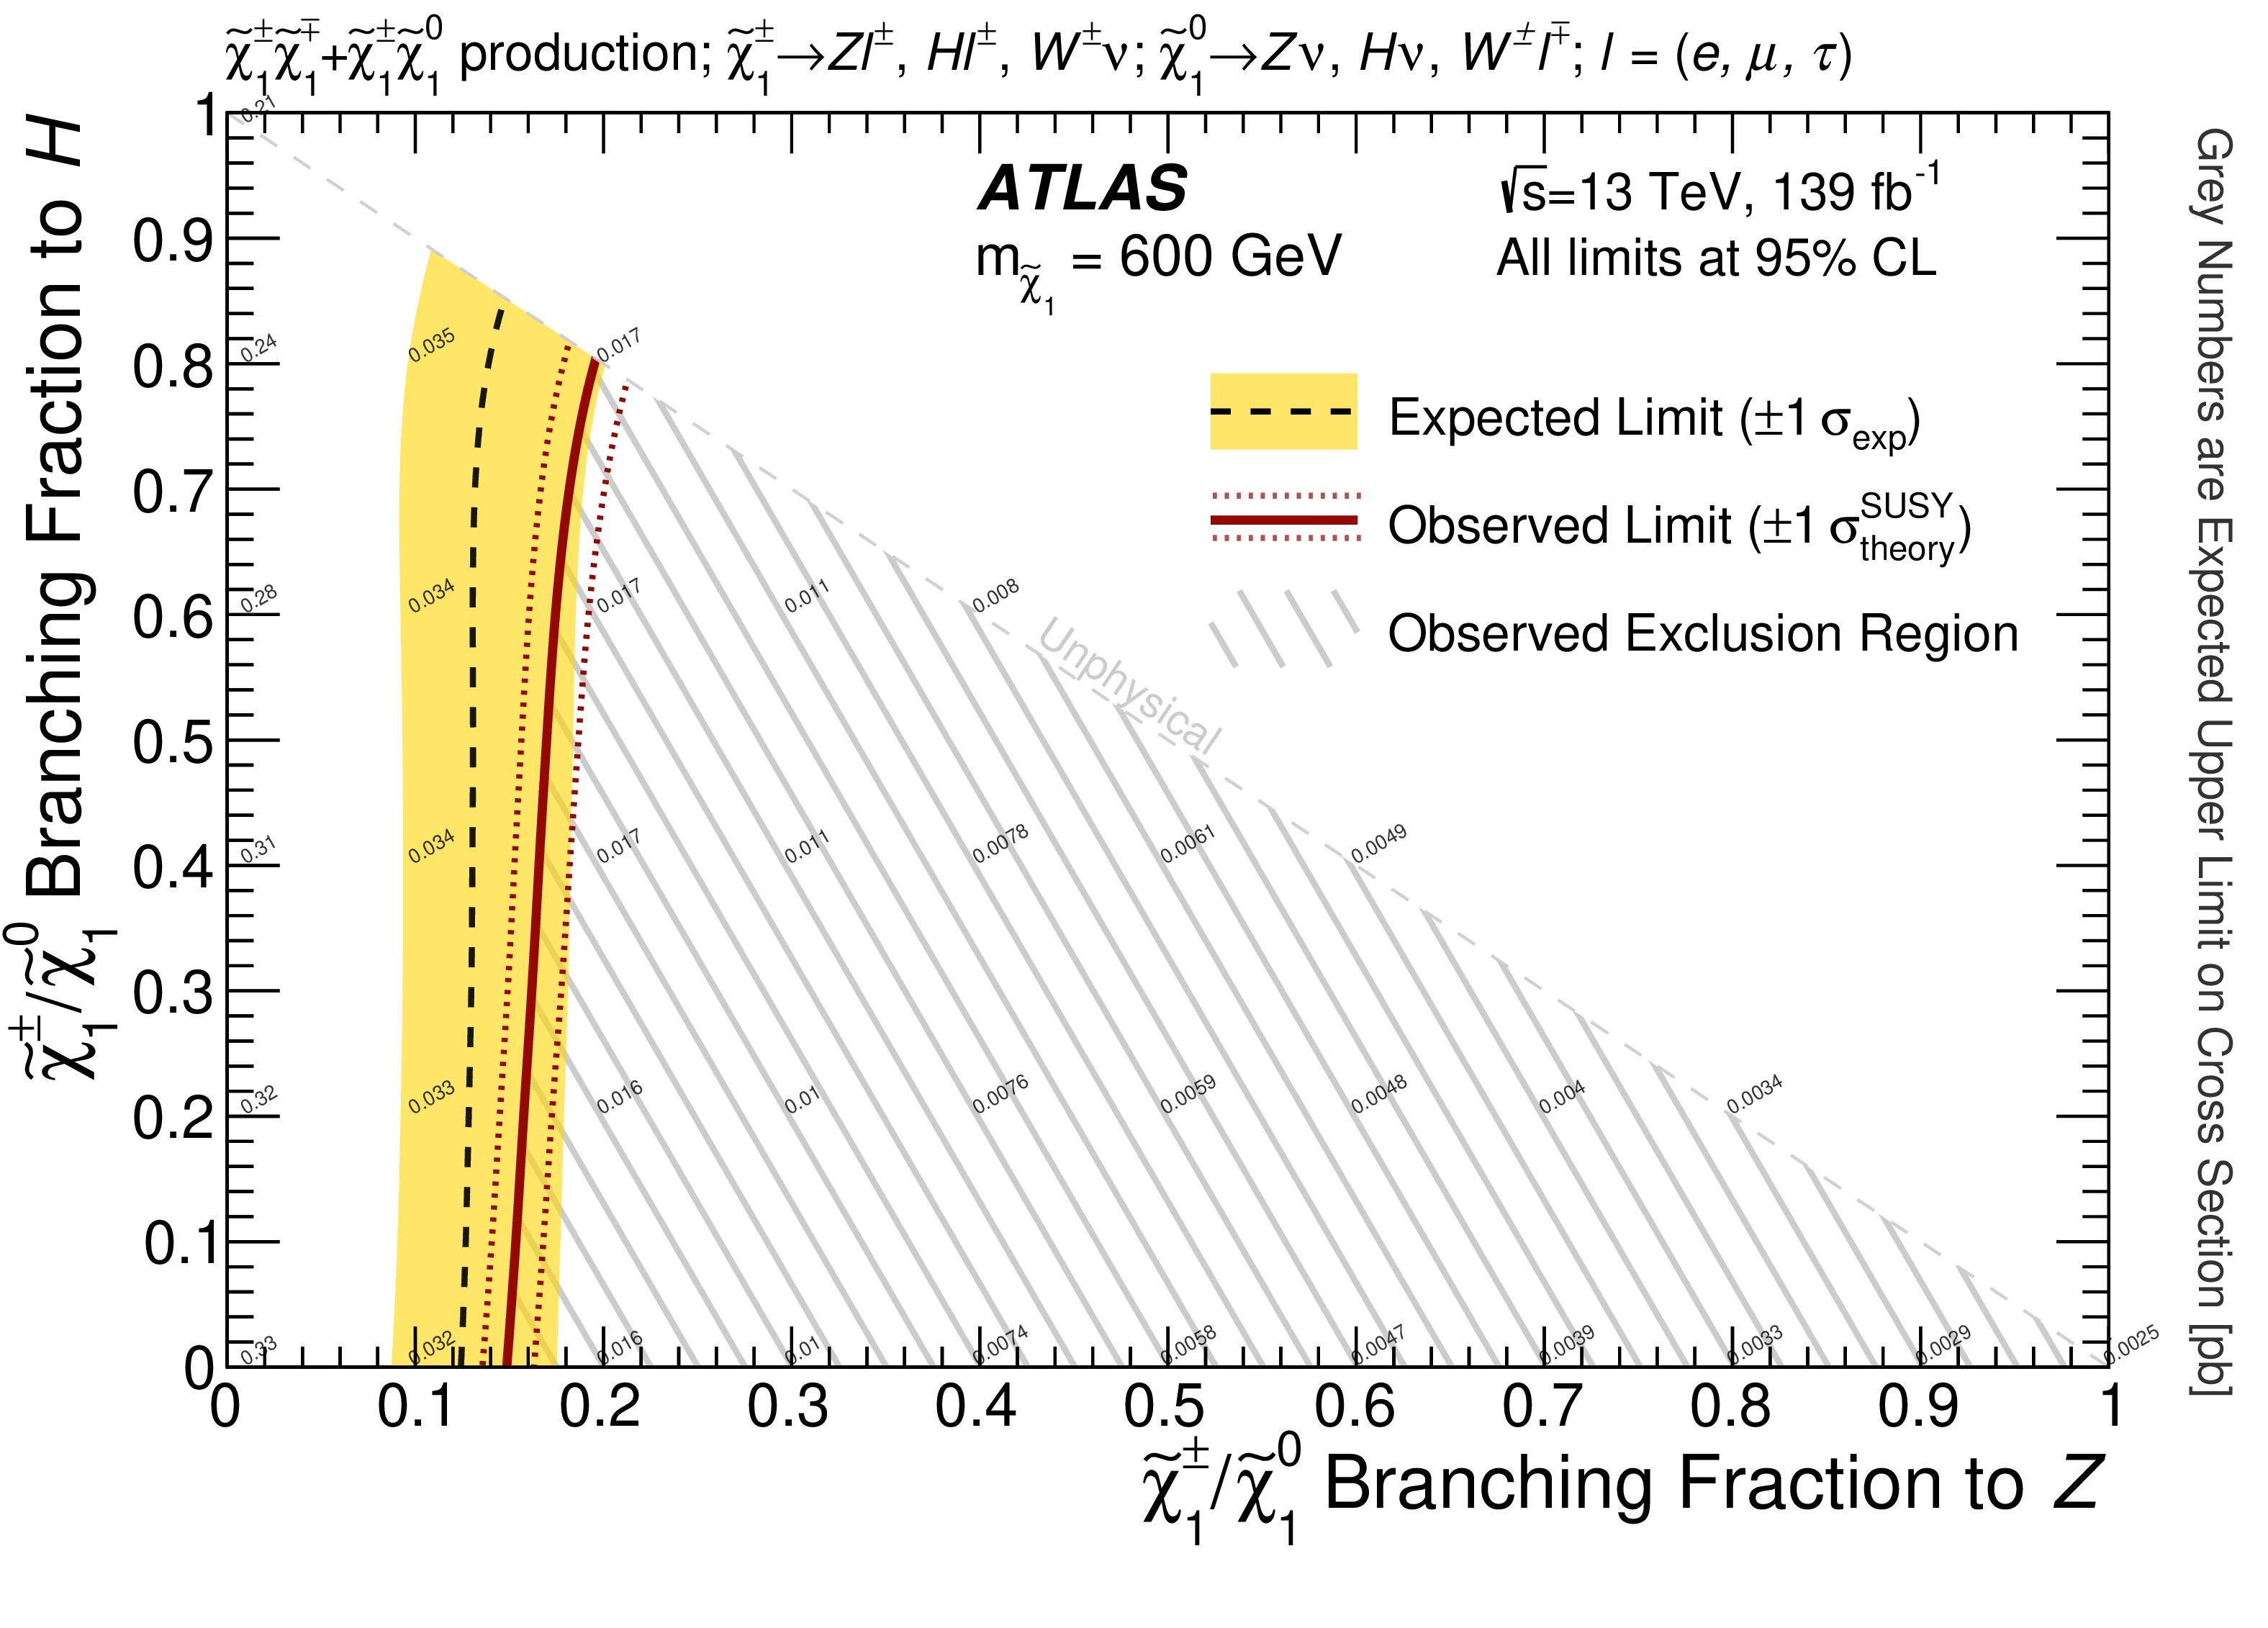
\includegraphics[width=0.98\textwidth]{figs/rpvthreel/triangleLimits_bre_33_brm_33_brt_33_mass_600_GreyexpectedUpperLimit_XS.png}
%      \caption{}
%      \label{fig:triangle_democratic_UpperLimExpectedXS}
%    \end{subfigure}
%    \hfill
%    \begin{subfigure}[b]{0.49\textwidth}
%      \centering
%      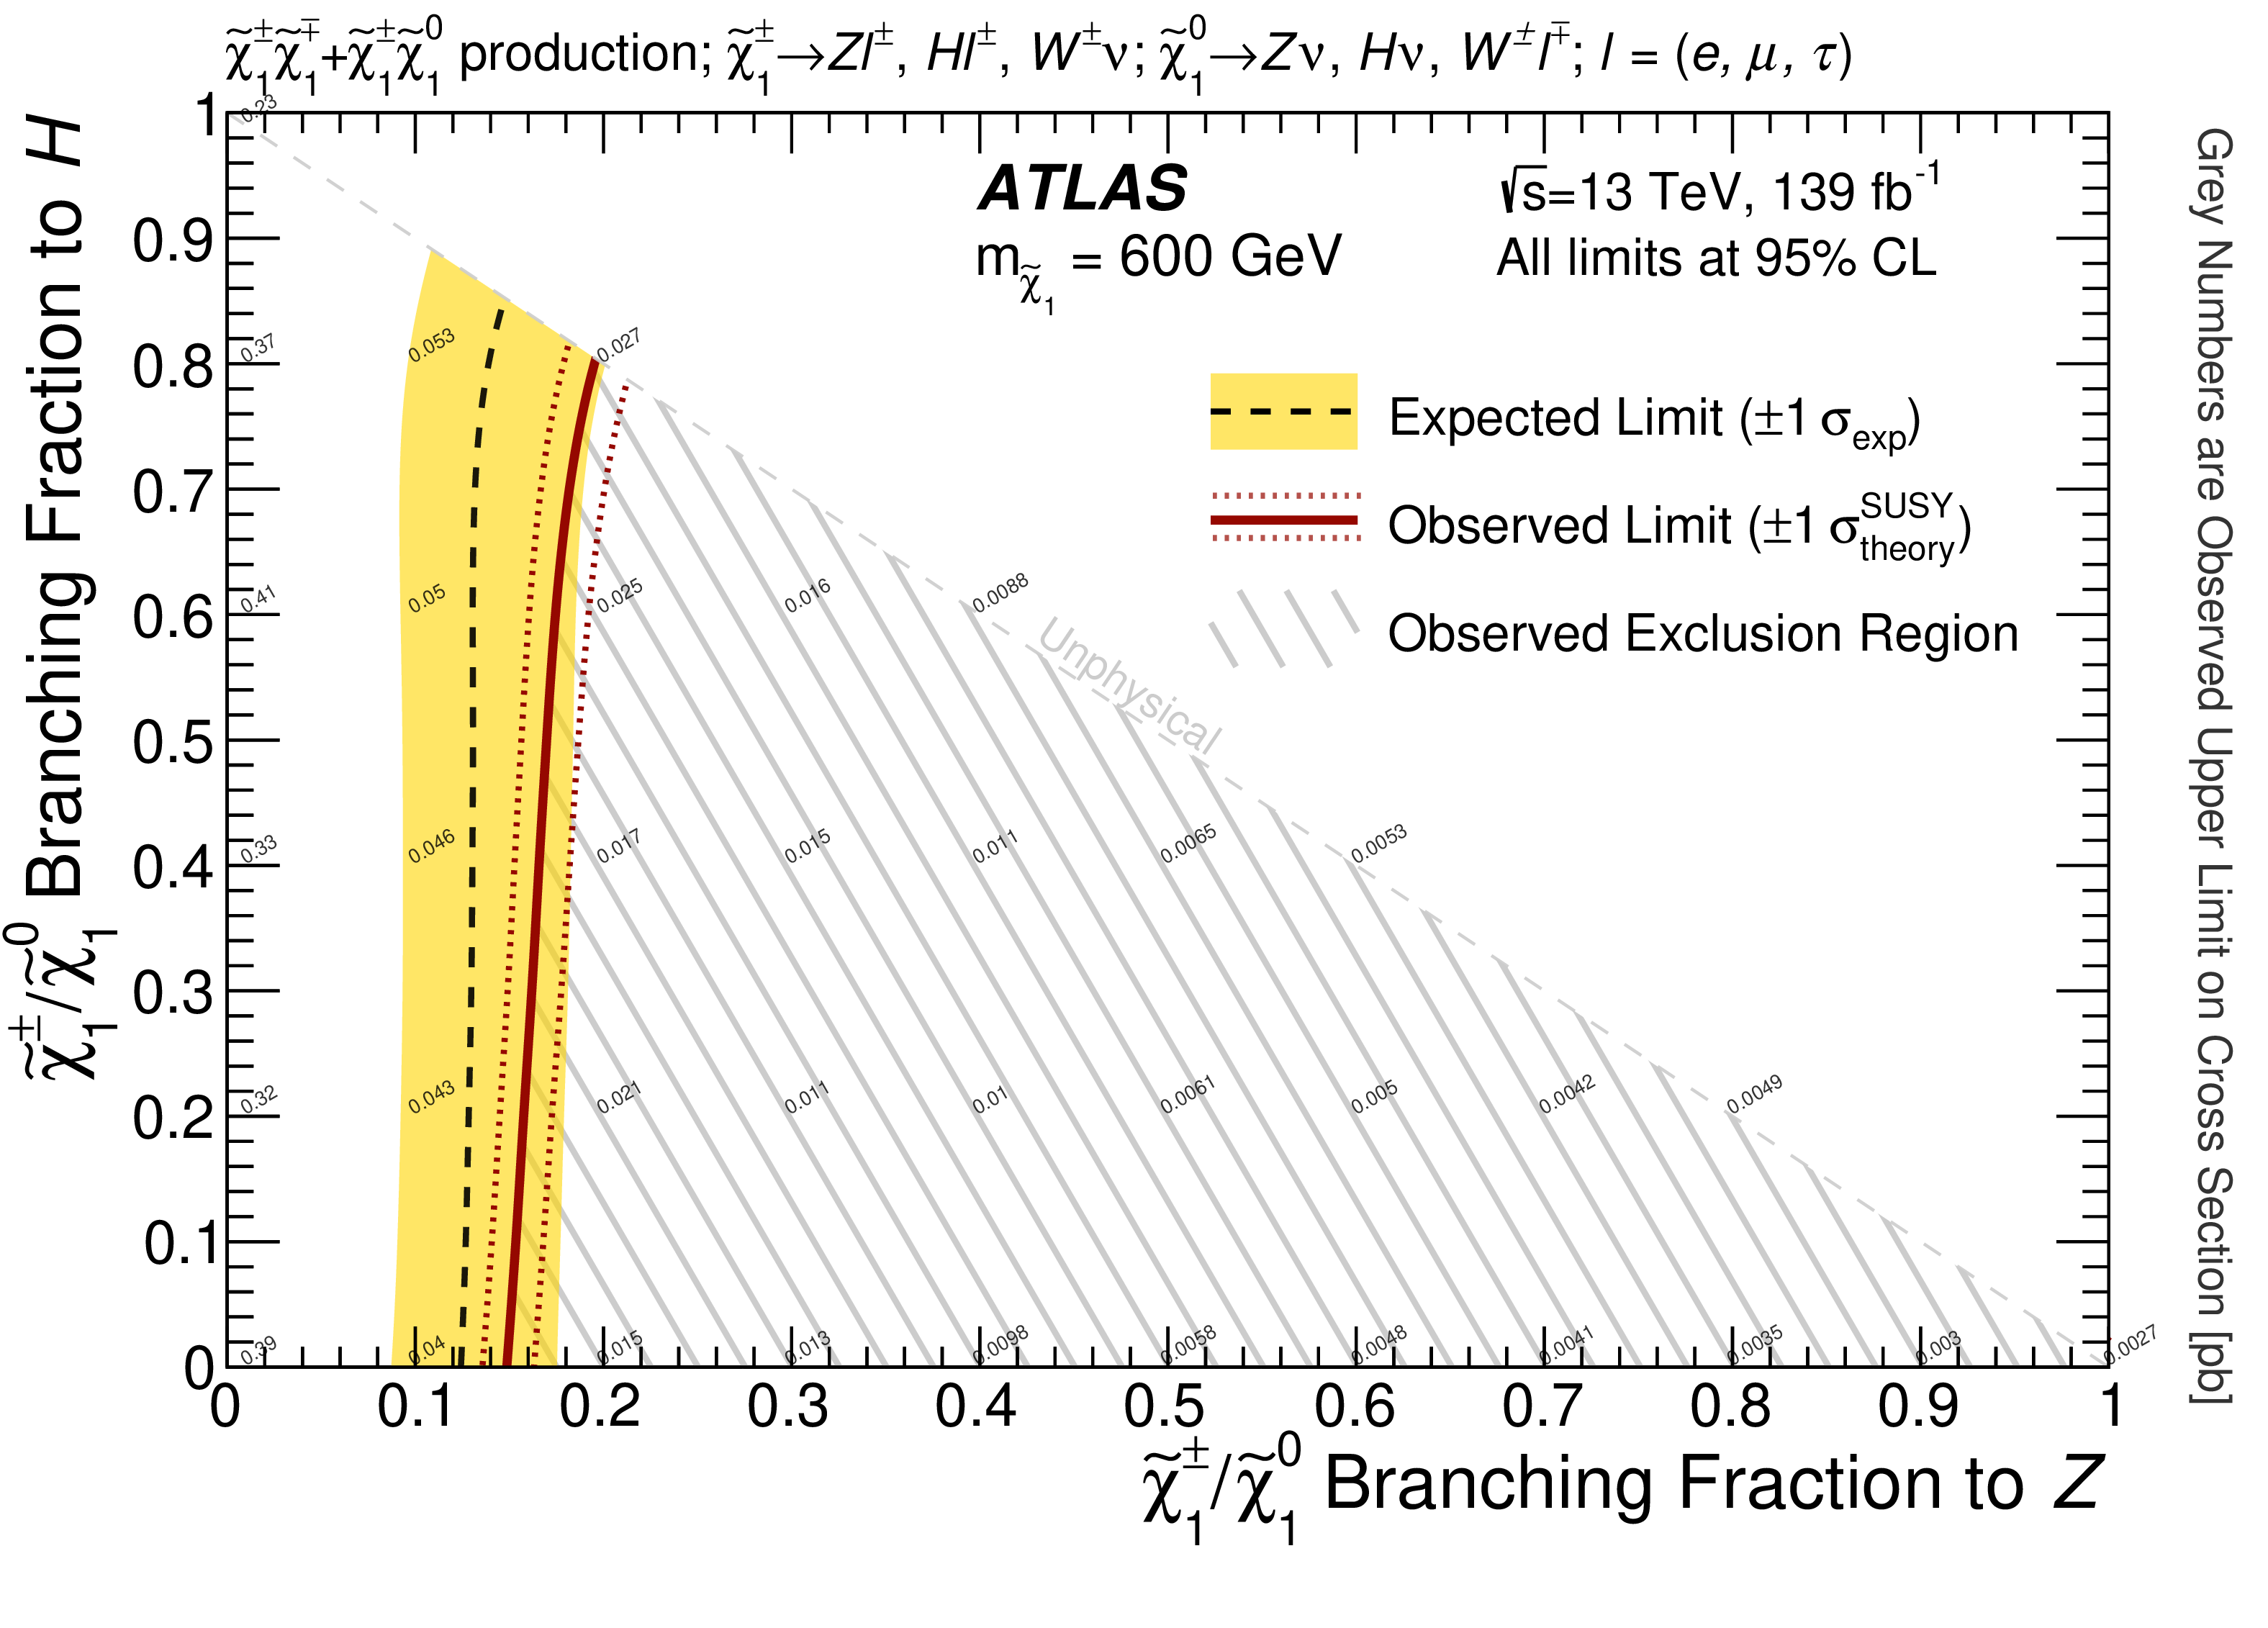
\includegraphics[width=0.98\textwidth]{figs/rpvthreel/triangleLimits_bre_33_brm_33_brt_33_mass_600_GreyupperLimit_XS.png}
%      \caption{}
%      \label{fig:triangle_democratic_UpperLimObservedXS}
%    \end{subfigure}
%    \caption[Caption]{Caption \cite{ATLAS:2020uer}}
%    \label{fig:triangle_democratic_UpperLim}
%\end{figure}
